\documentclass[9pt]{beamer}
%\PassOptionsToPackage[dvipsnames]{xcolor}
%\usepackage[dvipsnames]{xcolor}
\usepackage{tikz}
\usepackage{subfiles}
\usepackage{graphicx} 
\usepackage{hyperref}
\usepackage{multimedia}
\usepackage{subcaption}
\usepackage{amsmath}
\usepackage{pgf}
\usepackage{comment}


%\usepackage[table,xcdraw]{xcolor}  %to include tables with colors
\usepackage{pgfplots}


\setbeamertemplate{footline}[page number]
\mode<presentation>{
%\usetheme{Malmoe}
%\usetheme{Antibes}
%\usetheme{warsaw}
\usetheme{Frankfurt}  %%
%\usetheme{Dresden}
%\usetheme{Madrid}
%\usetheme{Malmoe} %
%\usetheme{Ilmenau}
}
%\setbeamertemplate{footline}[\insertframenumber]

%\newcommand*\oldmacro{}%
%\let\oldmacro\insertshorttitle%
%\renewcommand*\insertshorttitle{%
% \oldmacro\hfill%
% \insertframenumber\,/\,\inserttotlaframenumber}

\AtBeginSection[]
{
\begin{frame}<beamer>
\frametitle{Plan}
\tableofcontents[currentsection]
\end{frame}
}


\definecolor{secinhead}{RGB}{249,196,95}
\definecolor{titlebg}{RGB}{51,51,51}
\definecolor{orangecl}{RGB}{255,81,0}

\setbeamercolor{secsubsec}{fg=secinhead,bg=black}
\setbeamercolor{frametitle}{fg=orangecl,bg=titlebg}\setbeamercolor{structure}{bg=titlebg,fg=orangecl}

\makeatletter
\let\insertsupervisor\relax
\newcommand\supervisortitle{Supervisor }
\makeatletter
\let\insertsupervisorinst\relax
\newcommand\supervisorinsttitle{Supervisorinst}
\mode<all>
{
  \newcommand\supervisor[1]{\def\insertsupervisor{#1}}
  \titlegraphic{}
}
\mode<all>
{
  \newcommand\supervisorinst[1]{\def\insertsupervisorinst{#1}}
  \titlegraphic{}
}
\defbeamertemplate*{title page}{supdefault}[1][]
{
  \vbox{}
  \vfill
  \begingroup
    \centering
    
\includegraphics[width=0.25\linewidth]{ArcelorMittal_logo.png}
    \vskip1em\par
    \begin{beamercolorbox}[sep=8pt,center,#1]{title}
%      \usebeamerfont{title}
      \inserttitle\par%
      \ifx\insertsubtitle\@empty\relax%
      \else%
        \vskip0.25em%
        {%\usebeamerfont{subtitle}
        \usebeamercolor[fg]{subtitle}\insertsubtitle\par}%
      \fi%     
    \end{beamercolorbox}%
    \vskip1em\par
    \begin{beamercolorbox}[sep=8pt,center,#1]{author}
    Presented By:\\
%      \usebeamerfont{author}
      \textbf{\insertauthor} \\
%      \usebeamerfont{institute}
      \insertinstitute
    \end{beamercolorbox}
   %     \begin{beamercolorbox}{institute}
   %   \usebeamerfont{institute}\insertinstitute
   % \end{beamercolorbox}
    \ifx\insertsupervisor\relax\relax\else
    \begin{beamercolorbox}[sep=8pt,center,#1]{author}
%      \usebeamerfont{author}
      \supervisortitle: \\ \textbf{~\insertsupervisor} \\
%      \usebeamerfont{institute}
      \insertsupervisorinst
    \end{beamercolorbox}\fi
    %\begin{beamercolorbox}[sep=8pt,center,#1]{institute}
    %  \usebeamerfont{institute}\insertinstitute
    %\end{beamercolorbox}
    \begin{beamercolorbox}[sep=8pt,center,#1]{date}
%      \usebeamerfont{date}
      \insertdate
    \end{beamercolorbox}\vskip0.5em
    {\usebeamercolor[fg]{titlegraphic}\inserttitlegraphic\par}
  \endgroup
  \vfill
  
}
\setbeamertemplate{title page}[supdefault][colsep=-4bp,rounded=true,shadow=\beamer@themerounded@shadow]\makeatother

\title{Finite Element simulation of 2D metal strip in Hot-Dip galvanization Process}
%\subtitle{Reissner Mindlin Plate}
\author{Emayavaramban ELANGO}
\supervisor{PHAM Van Thang}
\supervisorinst{PHAM Van Thang }
\institute{\'Ecole centrale De Nantes}
\supervisorinst{ArcelorMittal Maizi\`eres Research SA }
\date{\today}


\begin{document}
%\title[Finite Element simulation of 2D metal strip in Hot-Dip galvanization Process]{FEM in plates}
%\author{Emayavaramban Elango}
%\institute[ECN]


%\begin{frame}
%\maketitle
%\end{frame}

\frame{\titlepage}

\begin{frame}
\frametitle{Table of Content}
\tableofcontents
\end{frame}
\section{Introduction}



\subsection{Hot-Dip Galvanization Process}
\begin{frame}
\frametitle{Hot-Dip Galvanization Process}
\begin{figure}[h!]
%\centering
%\minipage{1\textwidth}%
  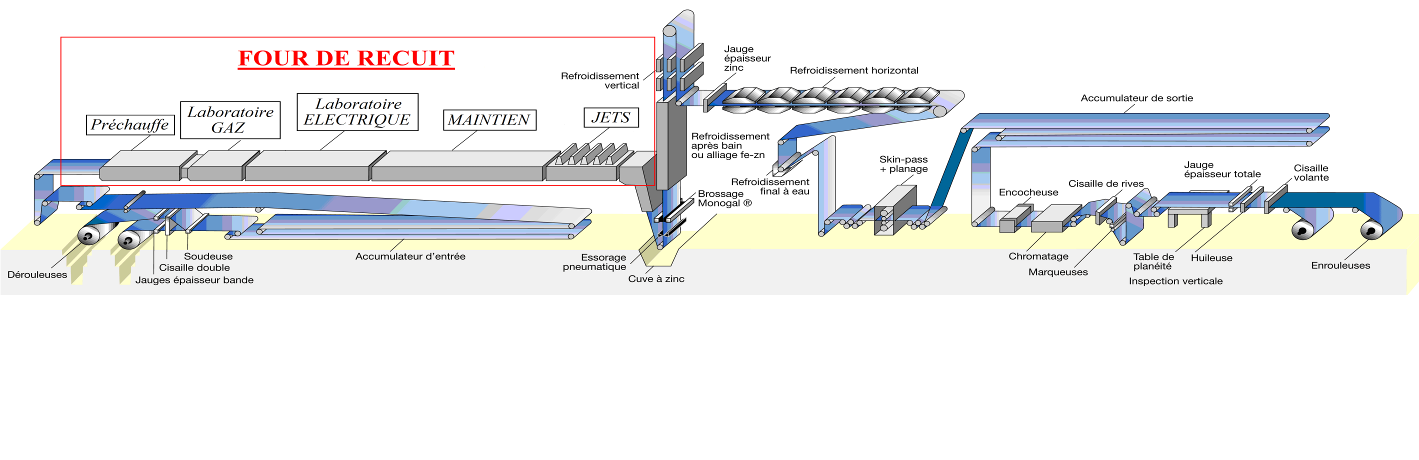
\includegraphics[width=1\linewidth,trim={0cm 4cm 0cm 0},clip]{galva_line.png}
 % \caption{FEM solution plot}\label{fig:awesome_image3}
%\endminipage
\end{figure}
\begin{columns}
\column{0.5\textwidth}

\begin{figure}[h!]
%\centering
%\minipage{1\textwidth}%
  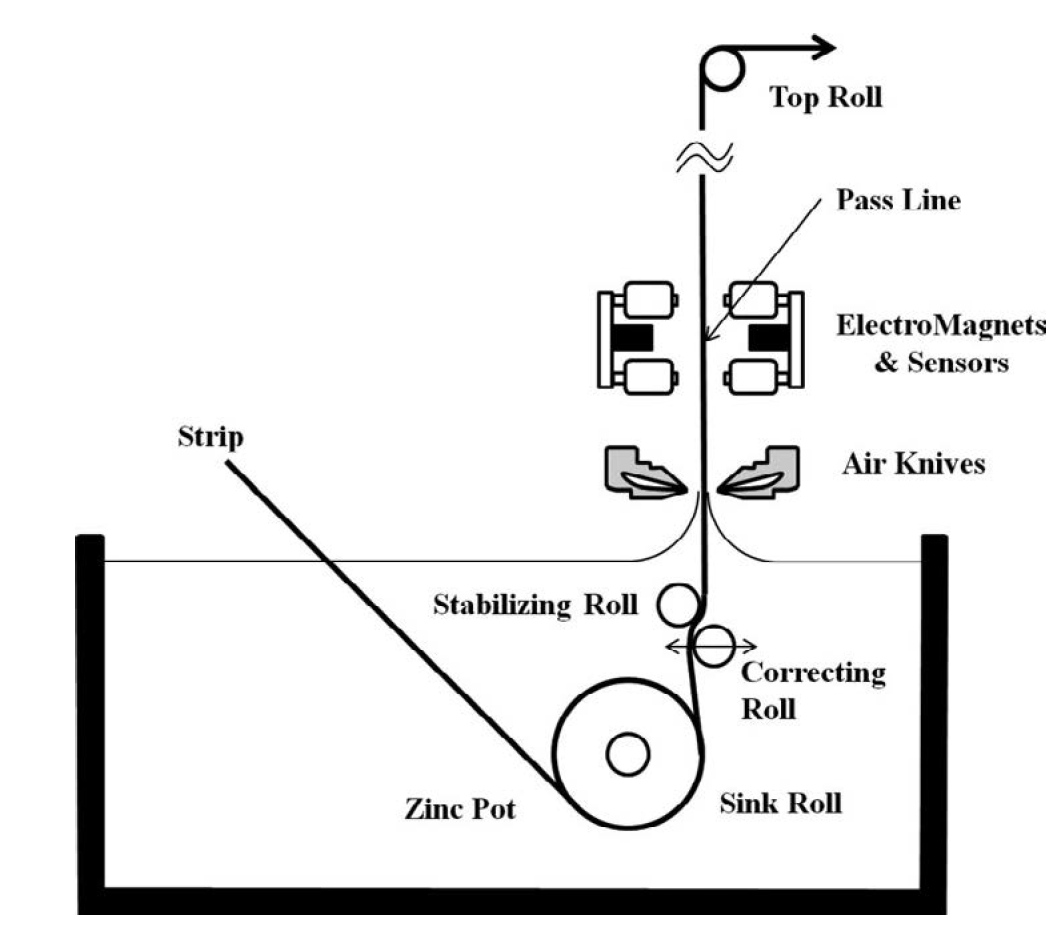
\includegraphics[width=1\linewidth,trim={0 0 0 1cm},clip]{hotdip.png}
 % \caption{FEM solution plot}\label{fig:awesome_image3}
%\endminipage
\end{figure}
\column{0.5\textwidth}
\begin{itemize}
\item A thin Layer of Zinc is coated to Increase the corrosion resistance of steel
\item Air knives control the thickness of the Zinc layer
\item Excessive Vibration results in uneven coating.
\item Electromagnets are used to control the  vibration of the strip. 
\end{itemize}
\end{columns}
\end{frame}




\begin{frame}
\frametitle{Finite Element Modelling}

In Finite element a  continuous domain is discretized into elements. Each element is connected by nodes.   
\begin{figure}[h!]
\centering
\minipage{0.8\textwidth}%
  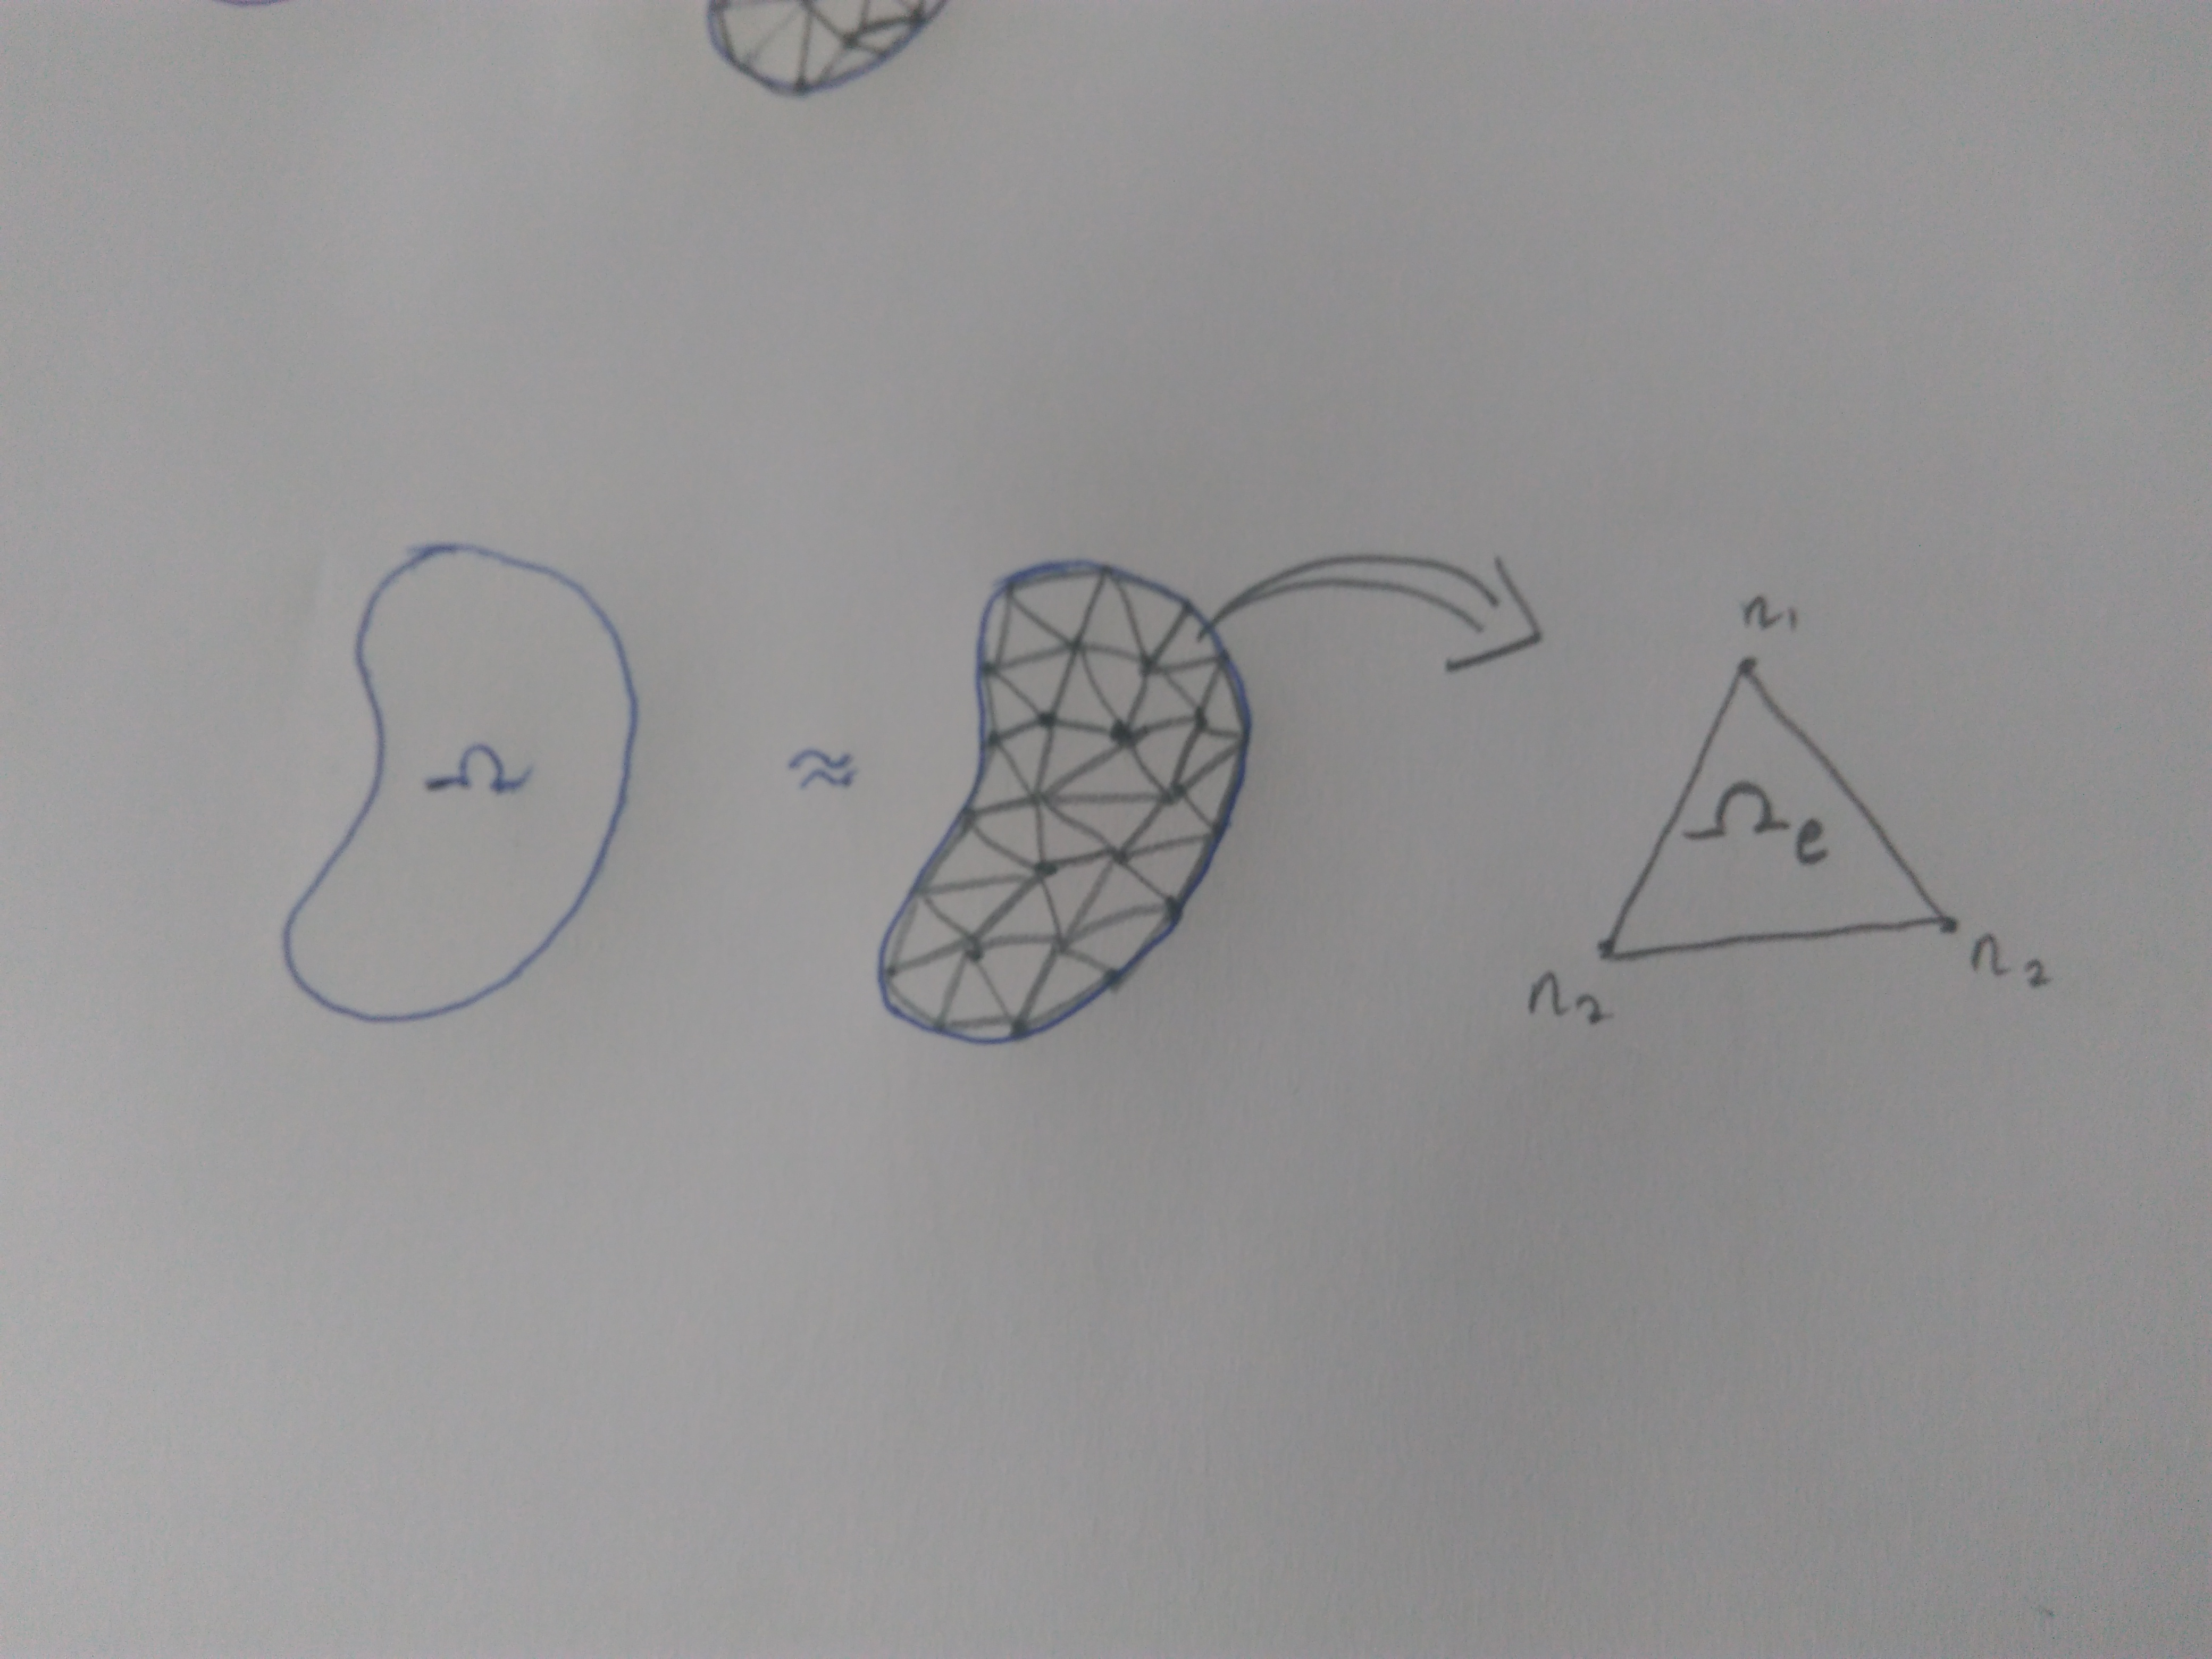
\includegraphics[width=\linewidth,trim={10cm 30cm 8cm 30cm},clip]{FEM.jpg}
  % \caption{FEM solution plot}
\endminipage
\end{figure} 
\begin{equation*}
\Omega \approx \sum_{i}^{nE} \Omega_e^i
\end{equation*}

\begin{itemize}
\item Complex behaviour of the metal strip.
\item Two dimensional domain and Three Dimensional Displacement field.
\item Complex and multiple boundary condition.
\item Free control over discretization of the domain.
\item Intuitive Solution Procedure.
\end{itemize}

\end{frame}

\section{Equation of Motion}

\begin{comment}

\begin{frame}
\frametitle{Description of Domain}

\begin{figure}[h!]
\centering
\subfile{domain.tex}
%\caption{NAS277} \label{NAS277sch}
\end{figure}
\begin{itemize}

\item $\Omega$ is the two dimensional domain strictly in xy plane 
\item $h$ is the thickness of the plate 
\item $\Omega_1$...$\Omega_i$ are the sub-domains where pressure forces $q_1$..$q_i$ are applied
\item $V$ is the Line speed and  $Nx$ is the tension on the line
\item $L$ is the length and  $W$ is the width 

\end{itemize}

\end{frame}



\begin{frame}
\frametitle{Description of Deformation (Reissner-Mindlin Plate Theory)}
A plate is a flat solid with uniform and smaller thickness than its other dimensions.A middle plane (Z=0) is equidistant from upper and lower faces.
\begin{block}{Assumptions (Thin and Thick Plate)}
\begin{itemize}
\item A point in the middle plane only moves vertically $u = 0$ and $v = 0 $
\item Thickness does not change during deformation.
\item only $\sigma_{33}$ is neglected (plane stress is assumed)
\item A line normal to the undeformed middle plane remains straight and not necessarily normal after deformation.
\end{itemize}
\end{block}


\begin{columns}
\column{0.5\textwidth}
\begin{figure}[h!]
%\centering
%\minipage{1\textwidth}%
  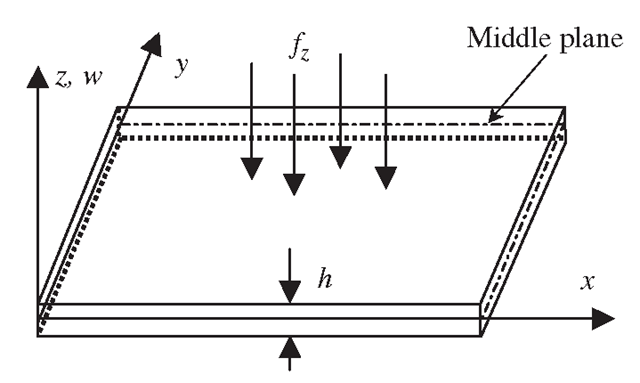
\includegraphics[width=1\linewidth,trim={0 0 0 1cm},clip]{plate.png}
 % \caption{FEM solution plot}\label{fig:awesome_image3}
%\endminipage
\end{figure}

\column{0.5\textwidth}


\begin{figure}[h!]
%\centering
%\minipage{1\textwidth}%
  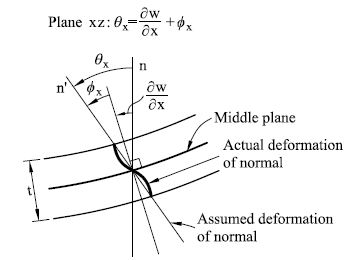
\includegraphics[width=1\linewidth,trim={0 0 0 0},clip]{RMplate.png}
 % \caption{FEM solution plot}\label{fig:awesome_image3}
%\endminipage
\end{figure}


\end{columns}

\end{frame}

\end{comment}
\begin{comment}

\begin{frame}
\frametitle{Theory of Plates}
\begin{block}{Kirchhoff Plate Theory}
\begin{itemize}
\item A line normal to the undeformed middle plane remains straight and normal after deformation.
\item Only for \textbf{Thin Plates} where $t/a \leq 0.1 $.
\item $\sigma_{23}$ and $\sigma_{13}$ are neglected.
\end{itemize}
\end{block}


\begin{figure}[h!]
%\centering
%\minipage{1\textwidth}%
  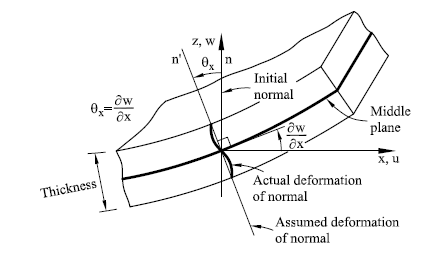
\includegraphics[width=0.6\linewidth,trim={0 0 0 0},clip]{Kplate.png}
 % \caption{FEM solution plot}\label{fig:awesome_image3}
%\endminipage
\end{figure}

\end{frame}


\begin{frame}
\frametitle{Theory of Plates (Reissner-Mindlin Plate Theory)}

\begin{block}{Reissner-Mindlin Plate Theory ( \textbf{Thin and Thin Plates} ) }
\begin{itemize}
\item A line normal to the undeformed middle plane remains straight and not necessarily normal after deformation.
\item For both \textbf{Thin and Thin Plates}.
%\item $\sigma_{23}$ and $\sigma_{13}$ are not neglected.
\end{itemize}
\end{block}


\begin{figure}[h!]
%\centering
%\minipage{1\textwidth}%
  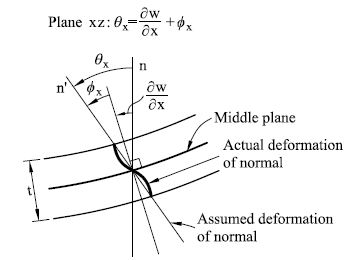
\includegraphics[width=0.6\linewidth,trim={0 0 0 0},clip]{RMplate.png}
 % \caption{FEM solution plot}\label{fig:awesome_image3}
%\endminipage
\end{figure}

\end{frame}

\end{comment}
\begin{comment}

\begin{frame}
\frametitle{Description of velocity}

\begin{columns}
\column{0.3\textwidth}
\begin{block}{Lagrangian}
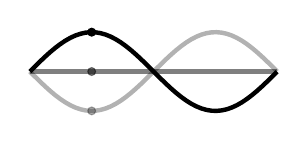
\begin{tikzpicture}[scale=0.5]

\draw [ultra thick,domain=0:2*3.14, samples=50] plot (\x, {+sin(\x r)});
\draw [ultra thick,domain=0:2*3.14, samples=50,opacity=0.5] plot (\x, {0});
\draw [ultra thick,domain=0:2*3.14, samples=50,opacity=0.3] plot (\x, {-sin(\x r)});

\draw[fill=black] (3.14*0.5,1,0) circle (0.1 );
\draw[fill=black,opacity=0.5] (3.14*0.5,0,0) circle (0.1 );
\draw[fill=black,,opacity=0.3] (3.14*0.5,-1,0) circle (0.1 );
 \end{tikzpicture}
 \begin{itemize}
 \item Material Point moves along with spatial point
 \item Used for solids
 \end{itemize}
\end{block}

\column{0.3\textwidth}
\begin{block}{Eulerian}


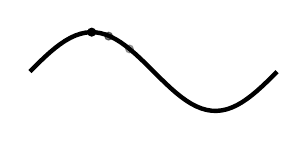
\begin{tikzpicture}[scale=0.5]

\draw [ultra thick,domain=0:2*3.14, samples=50] plot (\x, {3+sin(\x r)});
%\draw [ultra thick,domain=0:2*3.14, samples=50,opacity=0.7] plot (\x, {0});
%\draw [ultra thick,domain=0:2*3.14, samples=50,opacity=0.3] plot (\x, {-sin(\x r)});

\draw[fill=black] (3.14*0.5,3+1,0) circle (0.1 );
\draw[fill=black,opacity=0.5] (2,3+0.9,0) circle (0.1 );
\draw[fill=black,,opacity=0.3] (2.53,3+0.574,0) circle (0.1 );



 \end{tikzpicture}
 \begin{itemize}
 \item Material Point moves but spatial point stays
 \item Used for fluids
 \end{itemize}
 
 \end{block}
\column{0.3\textwidth}
\begin{block}{Mixed}


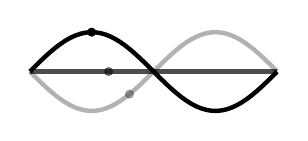
\begin{tikzpicture}[scale=0.5]


\draw [ultra thick,domain=0:2*3.14, samples=50] plot (\x, {-3+sin(\x r)});
\draw [ultra thick,domain=0:2*3.14, samples=50,opacity=0.7] plot (\x, {-3});
\draw [ultra thick,domain=0:2*3.14, samples=50,opacity=0.3] plot (\x, {-3-sin(\x r)});

\draw[fill=black] (3.14*0.5,-3+1,0) circle (0.1 );
\draw[fill=black,opacity=0.5] (2,-3,0) circle (0.1 );
\draw[fill=black,,opacity=0.3] (2.53,-3-0.574,0) circle (0.1 );

 \end{tikzpicture}
 \begin{itemize}
 \item Both point moves independently.
 \item Moving Material
 \end{itemize}
 
 \end{block}
 
\end{columns}
\begin{block}{Material Derivative}


\begin{equation*}
\frac{d(\circ)}{dt}=\frac{\partial(\circ)}{\partial t} + V_i \cdot (\circ)_{,i} 
\end{equation*}
\begin{equation*}
  v_i = \dot{u_i}+V_1u_{i,1}
\end{equation*} 

\end{block}

\end{frame}

\end{comment}

\subsection{Hamilton Principle}
\begin{frame}
\frametitle{Hamilton principle}
Hamilton principle is used to derive the equation of motion
and the Hamilton is given as 
 \begin{align*}
H  = \int_{t_0}^{t_1} \left( T - V + W \right) dt  
 \end{align*}
 The Hamilton Principle states that variation of Hamilton is zero
 \begin{align*}
 \delta H  =  \int_{t_0}^{t_1} \left( \delta T - \delta V + \delta W \right) dt     =  0 
 \end{align*}
 The variation of displacement $\delta u$ is zero at the beginning and end time.
 \begin{align*}
 \delta u \Big|_{t_0}^{t_1} = 0
 \end{align*}
 $T$ is the kinetic energy, $V$ in the potential energy and $W$ is the work done to the system.
 
\end{frame}





\begin{frame}
\frametitle{Final Equation of Motion}
\begin{block}{Final weak form}
\begin{equation*}
\begin{split}
 \int \int_\Omega 
\rho \ddot{\tilde{u_i}} Z_{ij} \delta {\tilde{u_i}}
+
2 \rho V_1 \delta {\tilde{u_i}} Z_{ij} \dot{\tilde{u}}_{j,1} 
-
\rho V_1^2 \tilde{u}_{j,1} Z_{ij} \delta \tilde{u}_{j,1}
\\ 
+
\kappa^T \tilde{D} \delta\kappa 
+
\left(\epsilon^S\right)^T \tilde{D_c} \delta\epsilon^S 
+ 
 w_{, \alpha} \tilde{\sigma}^A  \delta w_{, \alpha} d \Omega     
=  
 \sum_i^{nb}   \int  \int_{\Omega_i} q_i \mathbf{\delta u_i}  d \Omega_i dt
\end{split} 
\end{equation*}

\end{block}

\begin{block}{Final strong Form}

\begin{equation*}
\begin{split}
\rho h \left( \frac{\partial ^ 2 w}{\partial t ^ 2 }+2V_1\frac{\partial ^ 2 w}{\partial x \partial t} + V_1^2
\frac{\partial ^ 2 w}{\partial x ^ 2 } \right)  + D  \triangledown ^4 w - N_xh\frac{\partial ^ 2 w}{\partial x ^ 2 }=F 
\end{split} 
\end{equation*}


\end{block}
\begin{equation*}
\triangledown ^4 w = \frac{\partial ^ 4 w}{\partial x ^ 4 }+2 \frac{\partial ^ 4 w}{\partial x ^ 2 \partial y ^ 2 } + \frac{\partial ^ 4 w}{\partial Y ^ 4 } \qquad D = \frac{Eh^3}{12 \left( 1 - \nu^2 \right) }
\end{equation*}

Where, $\rho$ = Density, $N_x$ = Axial Stress, $h$ = thickness, $V_1$ = Line speed, $F$ = Distributed Force
\end{frame}

\section{Finite Element Formulation}


\begin{frame}
\frametitle{Shape function of a rectangular  element}

The displacement field over the element is given as the sum of product of shape function and nodal displacements. Here $n$ is the total number of nodes in an element

 \begin{columns}
 \column{0.6\textwidth}
\begin{block}{Displacement field of an element}
 \begin{equation*}
\begin{split}
\tilde{\mathbf{u}} \approx \sum_{i=1}^{n}\left(N_iw_i+\overline{N}_i\theta_{x_i} +\overline{\overline{N}}_i\theta_{y_i}\right)
\end{split}
\end{equation*}
\begin{equation*}
\begin{split}
\tilde{u} = \left[ w, \theta_x , \theta_y  \right]^T
\theta_x =\frac{\partial w}{\partial x}
 \theta_y  =\frac{\partial w}{\partial y}
\end{split}
\end{equation*}
\end{block}
 \column{0.4\textwidth}
%
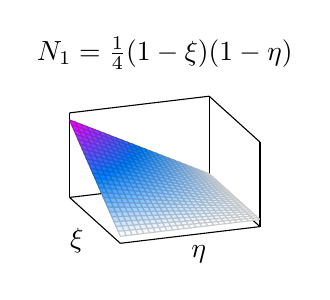
\begin{tikzpicture}
\pgfplotsset{compat=1.8,width=4cm,compat=newest}
  \begin{axis}[colormap/cool,
  title = {$N_1=\frac{1}{4}(1-\xi)(1-\eta)$},
  ticks=none,
  %axis x line*=box,axis y line*=box, 
  %axis z line=none, 
  				view/h=70,	
  				%,hide axis
  				%axis on top,
				%axis lines*=box, 
				  	 ,xlabel = $\xi$
     , ylabel = $\eta$, 				
  				]
    \addplot3[surf,
	domain=-1:1,
	domain y=-1:1,    
    ] {0.25*(1 - x - y + x*y)};
  \end{axis}
\end{tikzpicture}

\end{columns}


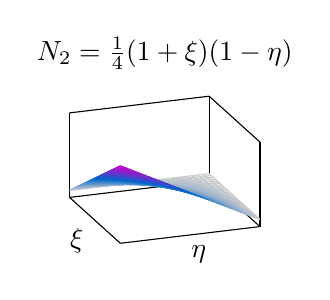
\begin{tikzpicture}
\pgfplotsset{compat=1.8,width=4cm,compat=newest}
  \begin{axis}[colormap/cool,
  	%hide axis,
  	view/h=70,
  	ticks=none,
  	title = { $N_2=\frac{1}{4}(1+\xi)(1-\eta)$ },
  	 xlabel = $\xi$
     , ylabel = $\eta$,
     axis lines*=box, 
  	]
    \addplot3[surf,
	domain=-1:1,
	domain y=-1:1,    
    ]  {0.25*(1 + x - y - x*y)};
  \end{axis}
 
  
\end{tikzpicture}
~
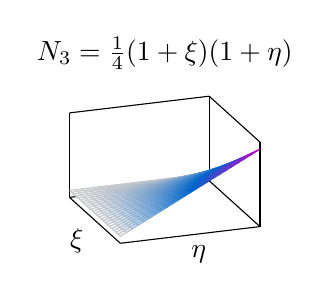
\begin{tikzpicture}
\pgfplotsset{compat=1.8,width=4cm,compat=newest}
  \begin{axis}[colormap/cool,
  %,hide axis
  view/h=70,
  ticks=none,
  title = { $N_3=\frac{1}{4}(1+\xi)(1+\eta)$ },
    	 xlabel = $\xi$
     , ylabel = $\eta$
  ,axis lines*=box,
   ]
    \addplot3[surf,
	domain=-1:1,
	domain y=-1:1,    
    ]  {0.25*(1 + x + y + x*y)};
  \end{axis}
\end{tikzpicture}
~
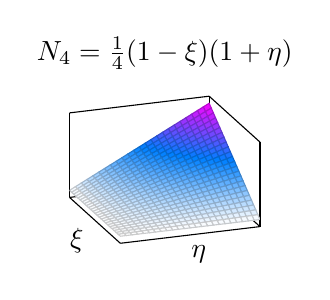
\begin{tikzpicture}
\pgfplotsset{compat=1.8,width=4cm,compat=newest}
  \begin{axis}[colormap/cool,
  %,hide axis,
  view/h=70,
  ticks=none,
  title = { $N_4=\frac{1}{4}(1-\xi)(1+\eta)$ },
    	 xlabel = $\xi$
     , ylabel = $\eta$
    ,axis lines*=box,
  ]
    \addplot3[surf,
	domain=-1:1,
	domain y=-1:1,    
    ]  {0.25*(1 - x + y - x*y)};
  \end{axis}
\end{tikzpicture}



\end{frame}


\begin{frame}
\frametitle{Representation of Displacements and Strains in terms of Shape Function.}
The FE approximation 
\begin{equation*}
\tilde{\mathbf{u}} \approx \sum_{i=1}^{n}\left(N_iw_i+\overline{N}_i\theta_{x_i}+\overline{\overline{N}}_i\theta_{y_i}\right)
\end{equation*}
is written in matrix format as
\begin{equation*}
\tilde{\mathbf{u}} \approx 
\begin{bmatrix}
N_1 & 0 & 0  & \cdots & N_{nN} & 0 & 0 \\
0 & \overline{N}_1 & 0  & \cdots & 0 & \overline{N}_{nN} & 0 \\
0 & 0 & \overline{\overline{N}}_1 & \cdots & 0 & 0 & \overline{\overline{N}}_{nN} \\
\end{bmatrix}
\left\{
\begin{array}{r}
w_1 \\
\theta_{x_1} \\
\theta_{y_1} \\
\vdots \\
w_{nN} \\
\theta_{x_{nN}} \\
\theta_{y_{nN}} \\
\end{array} \right\}
=
\mathbf{N} \tilde{\mathbf{u}}^e 
\end{equation*}
Similarly other terms of the Finite Element Matrices are
%\begin{equation*}
\begin{align*}
\dot{\tilde{ \mathbf{ u}} } & \approx  \mathbf{N}  \dot{\tilde{\mathbf{u}}}^e
&  
\ddot{\tilde{ \mathbf{ u}} } &  \approx   \mathbf{N}  \ddot{\tilde{\mathbf{u}}}^e
&
\mathbf{ \kappa } & \approx   \mathbf{ B } \tilde{\mathbf{u}}^e
&
\tilde{\mathbf{\epsilon}}^S  & \approx  \mathbf{ B_S }\tilde{\mathbf{u}}^e
\\
\tilde{u}_{1, \alpha}  & \approx  \mathbf{ H_A }\tilde{\mathbf{u}}^e
&
\tilde{u}_{\alpha, 1}  & \approx  \mathbf{ H_v }\tilde{\mathbf{u}}^e
&
\tilde{w}  & \approx  \mathbf{ N_f }\tilde{\mathbf{u}}^e
\end{align*}
%\end{equation*}
\end{frame}






\begin{frame}
\frametitle{Weak Form to FE format}
The Finite Element Matrix equation is given as
\begin{equation*}
\begin{split} 
\int \int_\Omega 
\left(
\rho
\left[ \mathbf{N}  \right]
\left[ \mathbf{Z}  \right]
\left[ \mathbf{N}  \right] 
\{ \ddot{\tilde{\mathbf{u}}}^e \}
\right) 
\delta \tilde{\mathbf{u}}^e
+
\left( 
2 \rho V_1
\left[ \mathbf{N}  \right]
\left[ \mathbf{Z}  \right]
\left[ \mathbf{H_v}  \right] 
\{ \dot{\tilde{\mathbf{u}}}^e \}
\right) 
\delta \tilde{\mathbf{u}}^e \\
-
\left( 
 \rho V_1^2
\left[ \mathbf{H_v}  \right]
\left[ \mathbf{Z}  \right]
\left[ \mathbf{H_v}  \right] 
\{\tilde{\mathbf{u}}^e \}
\right) 
\delta \tilde{\mathbf{u}}^e  
+
\left( 
\left[ \mathbf{B}  \right]
\left[ \mathbf{\tilde{D}}  \right]
\left[ \mathbf{B}  \right] 
\{\tilde{\mathbf{u}}^e \}
\right) 
\delta \tilde{\mathbf{u}}^e  \\
+
\left( 
\left[ \mathbf{B_S}  \right]
\left[ \mathbf{\tilde{D}_S}  \right]
\left[ \mathbf{B_S}  \right] 
\{\tilde{\mathbf{u}}^e \}
\right) 
\delta \tilde{\mathbf{u}}^e
+
\left( 
\left[ \mathbf{H_A}  \right]
\left[ \mathbf{\tilde{N}_A}  \right]
\left[ \mathbf{H_A}  \right] 
\{\tilde{\mathbf{u}}^e \}
\right) 
\delta \tilde{\mathbf{u}}^e
d \Omega
   \\
 =   
 \sum_i^{nb}   \int  \int_{\Omega_i} 
\left(  
 q_i 
\left[ \mathbf{\tilde{N}_f}  \right] 
\right)  
\delta \tilde{\mathbf{u}}^e
  d \Omega_i  
\end{split} 
\end{equation*}
After rearranging them to their respective groups we get.
\begin{equation*}
\left[ \mathbf{M}^e  \right] 
\{ \ddot{\mathbf{u}}^e \}
+
\left[ \mathbf{C}^e  \right] 
\{ \dot{\mathbf{u}}^e \}
+
\left[ \mathbf{K}^e  \right] 
\{\mathbf{u}^e \}
=
\{ \mathbf{F}^e \}
\end{equation*}

All the Element mass Matrices $\left[ \mathbf{M^e}  \right]$ are assembled in the final Mass Matrix $\left[ \mathbf{M} \right]$.Doing same for other matrices gives us the ODE in terms of FE matrices.
\begin{equation*}
\left[ \mathbf{M}  \right] 
\{ \ddot{\mathbf{u}} \}
+
\left[ \mathbf{C}  \right] 
\{ \dot{\mathbf{u}} \}
+
\left[ \mathbf{K}  \right] 
\{\mathbf{u} \}
=
\{ \mathbf{F} \}
\end{equation*}
\end{frame}


\begin{comment}
\begin{frame}
\frametitle{FEM matrices}

\begin{align*}
&\left[ \mathbf{M}^e  \right]  
= \rho
\int \int_\Omega 
\left(
\left[ \mathbf{N}  \right]
\left[ \mathbf{Z}  \right]
\left[ \mathbf{N}  \right] 
\right)  d \Omega  \\
&\left[ \mathbf{C}^e  \right]   
= 2 \rho V_1
\int \int_\Omega 
\left( 
\left[ \mathbf{N}  \right]
\left[ \mathbf{Z}  \right]
\left[ \mathbf{H_v}  \right] 
\right)  d \Omega  \\ &
\left[ \mathbf{K} ^e \right] 
=  - \rho V_1^2
\int \int_\Omega 
\left( 
\left[ \mathbf{H_v}  \right]
\left[ \mathbf{Z}  \right]
\left[ \mathbf{H_v}  \right] 
\right)  d \Omega + 
\int \int_\Omega  
\left[ \mathbf{B}  \right]
\left[ \mathbf{\tilde{D}}  \right]
\left[ \mathbf{B}  \right]  
  d \Omega   \\  &  \quad +
  \int \int_\Omega  
\left[ \mathbf{B_S}  \right]
\left[ \mathbf{\tilde{D}_S}  \right]
\left[ \mathbf{B_S}  \right] 
  d \Omega +
  \int \int_\Omega  
\left[ \mathbf{H_A}  \right]
\left[ \mathbf{\tilde{N}_A}  \right]
\left[ \mathbf{H_A}  \right]  
  d \Omega  \\ &
\{ \mathbf{F}^e \}  = 
 \sum_i^{nb}   \int  \int_{\Omega_i}   
 q_i 
\left[ \mathbf{\tilde{N}_f}  \right] 
  d \Omega_i    
\end{align*}

All the Element mass Matrices $\left[ \mathbf{M^e}  \right]$ are assembled in the final Mass Matrix $\left[ \mathbf{M} \right]$. Which gives us the  ODE in terms of FE matrices.

\begin{equation*}
\left[ \mathbf{M}  \right] 
\{ \ddot{\mathbf{u}} \}
+
\left[ \mathbf{C}  \right] 
\{ \dot{\mathbf{u}} \}
+
\left[ \mathbf{K}  \right] 
\{\mathbf{u} \}
=
\{ \mathbf{F} \}
\end{equation*}
\end{frame}



\end{comment}

\begin{frame}
\frametitle{Solution Procedure}
\textbf{Static Analysis:}\\

To solve a static system  
\begin{equation*}
 \left[ \mathbf{K}  \right] 
\{\mathbf{u} \}
=
\{ \mathbf{F} \} 
\end{equation*}
 $ u=K \backslash F $ command is used since, $u=K^{-1}F$ is a very expensive command. $u=K \backslash F$ command first factorizes the K matrix into upper and lower triangles then it is solved, which is a much more efficient process.
\\ 
\textbf{Modal Analysis:}\\ 


\begin{equation*}
\mathbf{M}\mathbf{\ddot{{ u}}}+\mathbf{K}\mathbf{{ u}}=0
\end{equation*}
is converted in to a eigenvalue  problem
\begin{equation*}
\left( \mathbf{K} - \omega^2 \mathbf{M}  \right) \overline{\mathbf{u} } = 0 \qquad { \mathbf{u}}=\overline{ \mathbf{u}}e^{i\omega t}
\end{equation*}
$\omega$ is the natural frequency and $\overline{\mathbf{u}}$ is the natural mode. In MATLAB, [V,D]=eig(K,M) function is used to do the modal analysis.
\end{frame}

\begin{frame}
\textbf{Dynamic Analysis:}\\
To solve the dynamic system
\begin{equation*}
\left[ \mathbf{M}  \right] 
\{ \ddot{\mathbf{u}} \}
+
\left[ \mathbf{C}  \right] 
\{ \dot{\mathbf{u}} \}
+
\left[ \mathbf{K}  \right] 
\{\mathbf{u} \}
=
\{ \mathbf{F} \}
\end{equation*}
Newmark time integration scheme is employed. 
\begin{block}{Newmark algorithm}
\begin{equation*}
R=F_t + \mathbf{M} \left(a_0 u_{t}+a_2 \dot{u}_{t} + a_3 \ddot{u}_{t} \right) + \mathbf{C} \left(a_1 u_{t}+a_4 \dot{u}_{t} + a_5 \ddot{u}_{t} \right) 
\end{equation*}
\begin{align*}
u_{t+1} & =\left[a_0 \mathbf{M} + a_1 \mathbf{C} + \mathbf{K} \right] ^ {-1} R \\
\dot{u}_{t+1} & =a_1 \left( u_{t+1} - u_{t} \right) - a_4 \dot{u}_t -a_5 \ddot{u}_t \\
\ddot{u}_{t+1} & =a_0 \left( u_{t+1} - u_{t}\right) - a_2 \dot{u}_t -a_3 \ddot{u}_t
\end{align*}
\end{block}
\begin{columns}
\column{0.7\textwidth}
$a_0$ .. $a_5$ are the integration variables which depends on the Integration parameters $\theta$, $\alpha$ and time step size $h$. 
$u_t$,$\dot{u}_t$ and $\ddot{u}_t$ are the displacement , velocity and acceleration of current time step. $u_{t+1}$,$\dot{u}_{t+1}$ and $\ddot{u}_{t+1}$ are the displacement , velocity and acceleration of next time step. 
\column{0.3\textwidth}
Unconditionally Stable for
\begin{align*}
\theta & \geq \frac{1}{2}  \\
\alpha & \geq \frac{1}{4}\left(\frac{1}{2}+\theta \right)^2
\end{align*}

\end{columns}
\end{frame}



\begin{frame}
\frametitle{Finite Element Discretization }
\begin{figure}[h!]
\centering

\begin{subfigure}{1\textwidth}

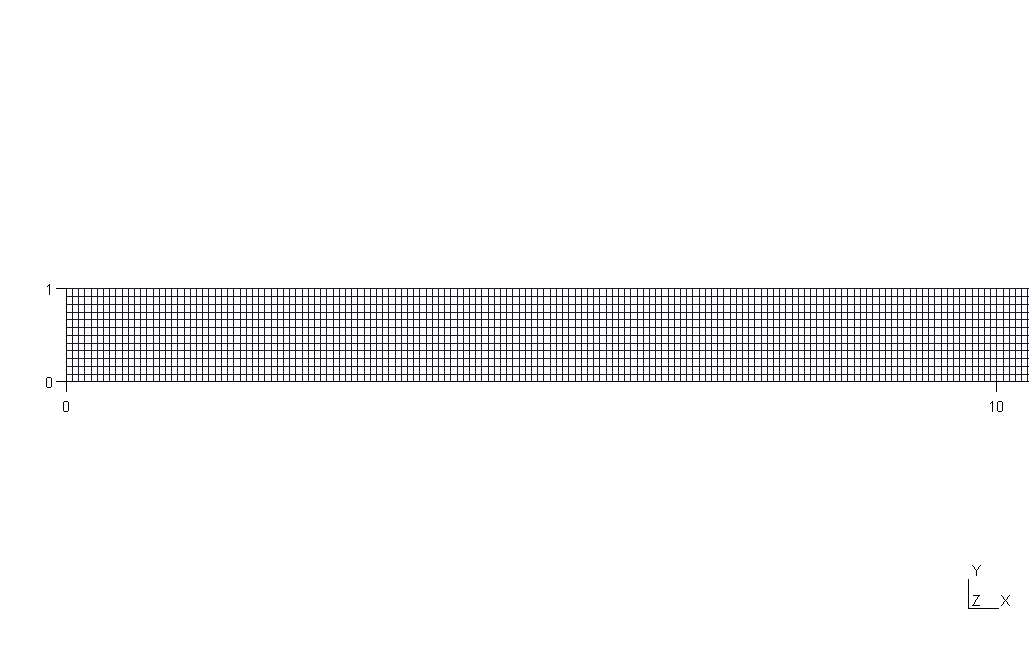
\includegraphics[width=\linewidth,trim={0cm 9cm 0cm 9cm},clip]{ParaStudy_onlydata/Mesh_Dependency/meshes/4_zoomed.png}
\caption{Mesh : $4$ , Nn = 7813, Solution Time = 929s }

\end{subfigure} \vfill


\begin{subfigure}{1\textwidth}

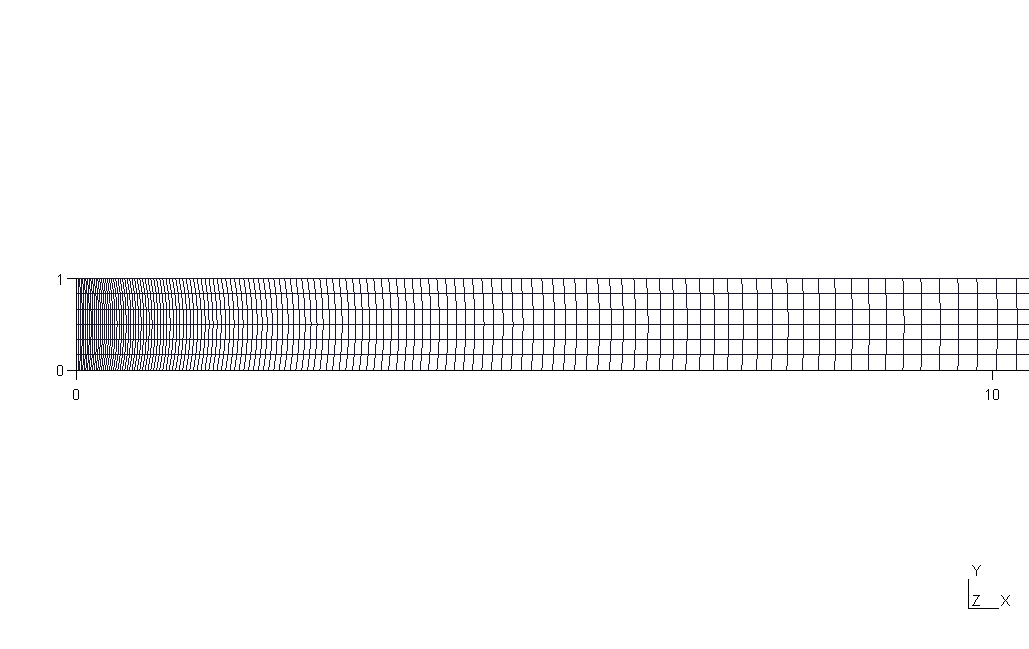
\includegraphics[width=\linewidth,trim={0cm 9cm 0cm 9cm},clip]{ParaStudy_onlydata/Mesh_Dependency/meshes/2_3_zoomed.png}
\caption{Mesh : $2\_3$ , Nn = 1407, Solution Time = 13s }

\end{subfigure} \vfill

\begin{subfigure}{1\textwidth}

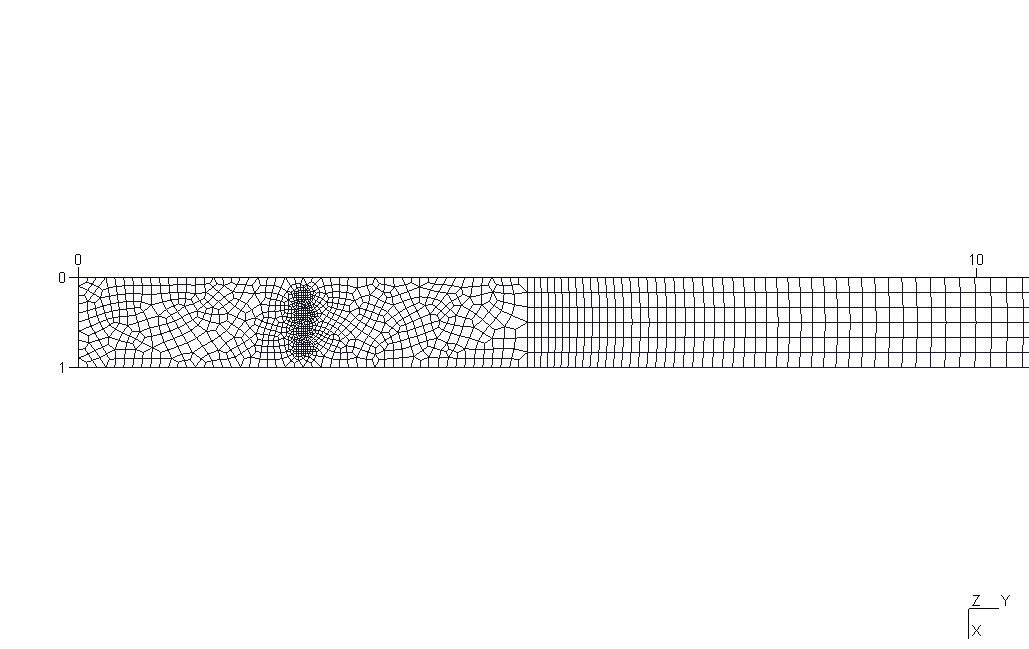
\includegraphics[width=\linewidth,trim={0cm 9cm 0cm 9cm},clip]{ParaStudy_onlydata/Mesh_Dependency/meshes/strip.png}
\caption{Mesh : strip , Nn = 1886, Solution Time = 21s }

\end{subfigure} 


\end{figure}
\end{frame}


\section{Verification Problems}

\begin{frame}
\frametitle{TIM69 Static Analysis , Circular Plate with Point load}

\begin{columns}
\column{0.5\textwidth}

\begin{figure}[h!]
\centering
\minipage{1\textwidth}%
  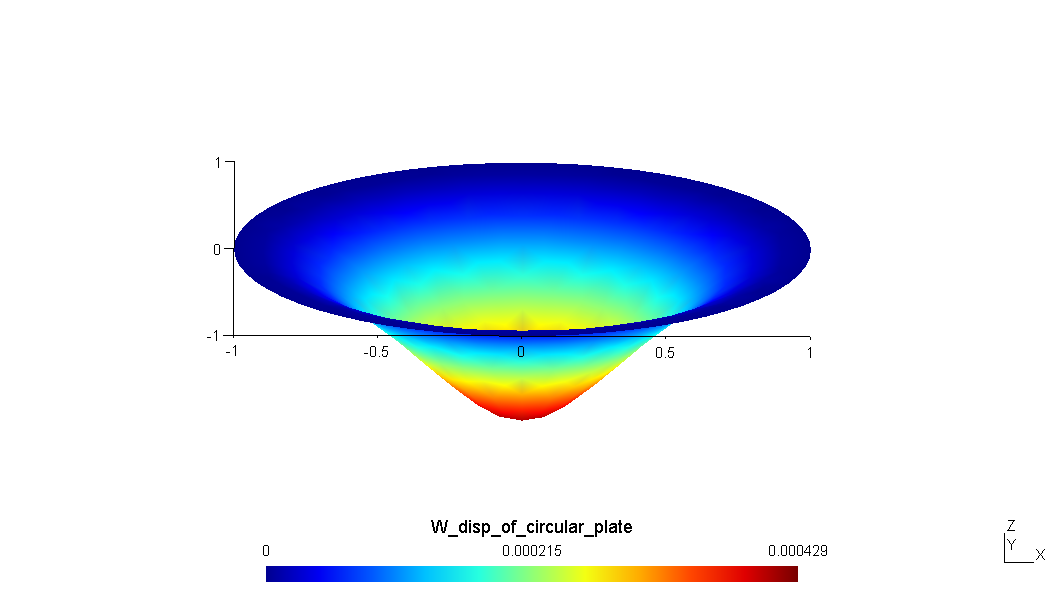
\includegraphics[width=\linewidth,trim={5cm 4cm 5cm 4cm},clip]{TIM69_pos.png}
  % \caption{FEM solution plot}
\endminipage
\end{figure}
The target analytically solution given as
\begin{equation}
w = \frac{F_z}{16 \pi D}\left[ r^2 - a^2 \right]+\frac{F_zr^2}{8 \pi D}\left[ log \frac{a}{r} \right]
\end{equation} 
 The analytical solution is -0.000434 $in$.\\ Numerical solution is $ -0.000429 in $. \\
So the Error percentage is $ 1.26 \% $. 
\column{0.5\textwidth}

\begin{table}[ht]
\renewcommand{\arraystretch}{1.5}
\centering
\begin{tabular}{ll}
\hline
\multicolumn{2}{l}{Material Property} \\ \hline  \hline
Young's Modulus ($E$)          & 5E11 $Pa$        \\
Poission's Ratio ($\nu$)       & 0.3            \\ 
    \hline
    \multicolumn{2}{l}{Geometric Data} \\ \hline  \hline
            Radius ($r$)        & 1 $m$   \\
            Thickness($t$)     &         0.01 $m$  \\
             \hline
    \multicolumn{2}{l}{Loading Data} \\ \hline  \hline
    Point Load ($F_z$)        & -1000 $N$     \\    \hline
\end{tabular}
\end{table}

\end{columns}


%\begin{table}[ht]
%\renewcommand{\arraystretch}{1.5}
%\centering
%\begin{tabular}{lll}
%\hline
%{Material } & {Geometric} & {Loading } \\ \hline  \hline
% ($E$)         = 5E11 $Pa$         & ($r$)       = 1 $m$        & ($F_z$) = -1000 $N$         \\
%($\nu$) = 0.3         &($h$)  = 0.01 $m$  &           \\ 
%            \hline
%\end{tabular}
%\end{table}

\begin{block}{Reference}
S.Timoshenko , S . Woinowsky , Theory of Plates and Shells , pg:69, Article : 19 . 
\end{block}

\end{frame}




\begin{frame}
\frametitle{VMP09 Modal Analysis , Free square Plate}

\begin{columns}
\column{0.5\textwidth}

\begin{figure}[h!]
\centering
\minipage{1\textwidth}%
  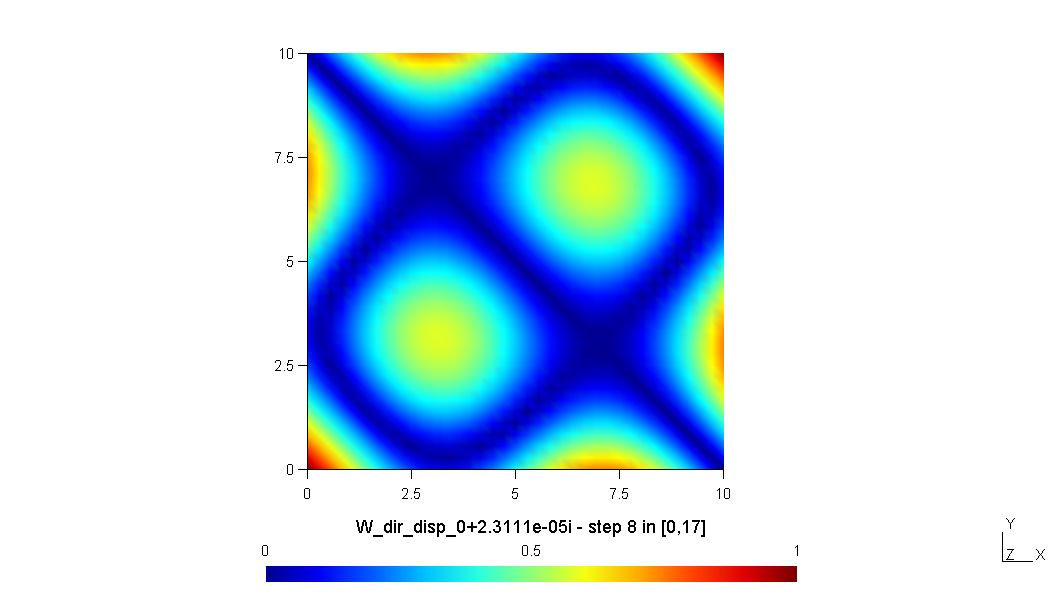
\includegraphics[width=\linewidth,trim={8cm 4cm 8cm 2cm},clip]{VMP09_T12_pos_F9.png}
  % \caption{FEM solution plot}
\endminipage
\end{figure}

The analytical frequency is 1.632 $Hz$. 
The numerical frequency is  1.626 $Hz$. \\
So the Error percentage is  0.32 $\%$ 


\column{0.5\textwidth}

\begin{table}[ht]
\renewcommand{\arraystretch}{1.5}
\centering
\begin{tabular}{ll}
\hline
\multicolumn{2}{l}{Material Property} \\ \hline  \hline
Young's Modulus ($E$)          &25E11 $Pa$        \\
Poission's Ratio ($\nu$)       & 0.3            \\ 
Density($\rho$)       &     8000         \\ 
    \hline
    \multicolumn{2}{l}{Geometric Data} \\ \hline  \hline
            length ($l$)        & 10 $m$   \\
            breath ($b$)        & 10 $m$   \\
            Thickness($t$)     &         0.01 $m$  \\
             \hline
\end{tabular}
\end{table}

\end{columns}



\begin{block}{Reference}
NAFEMS Manual. Solution Retrieved from Ansys verification problem (VMP09-T12).
\end{block}

\end{frame}



\begin{comment}

\begin{frame}
\frametitle{VMP09}

\begin{figure}[h!]
\begin{subfigure}{.3\textwidth}
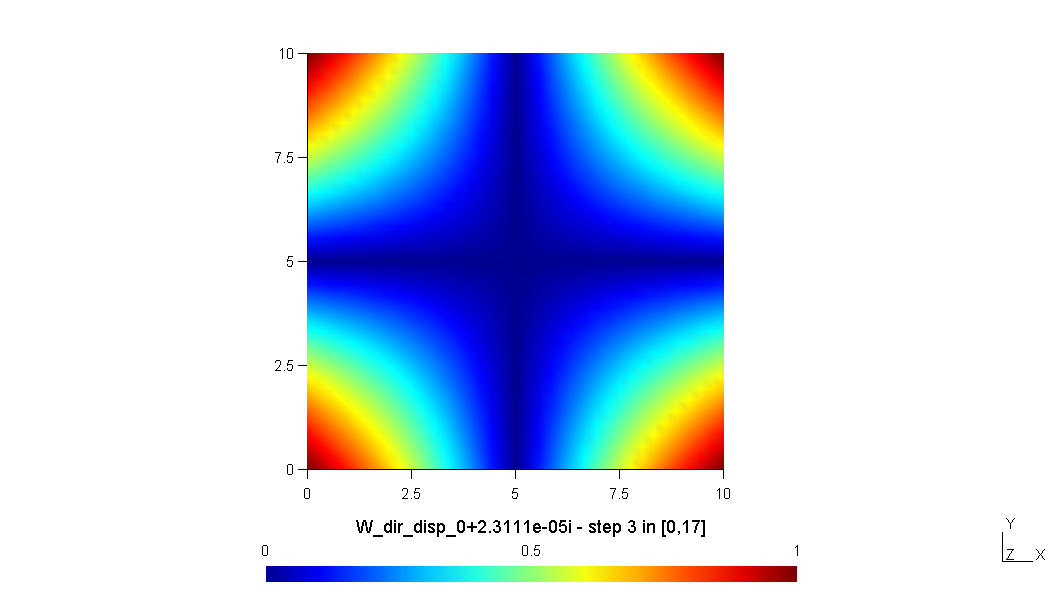
\includegraphics[width=\linewidth,trim={8cm 4cm 8cm 2cm},clip]{VMP09_T12_pos_F4.png}
%\caption{Mode Shape 4}
\end{subfigure} \hfill
\begin{subfigure}{.3\textwidth}
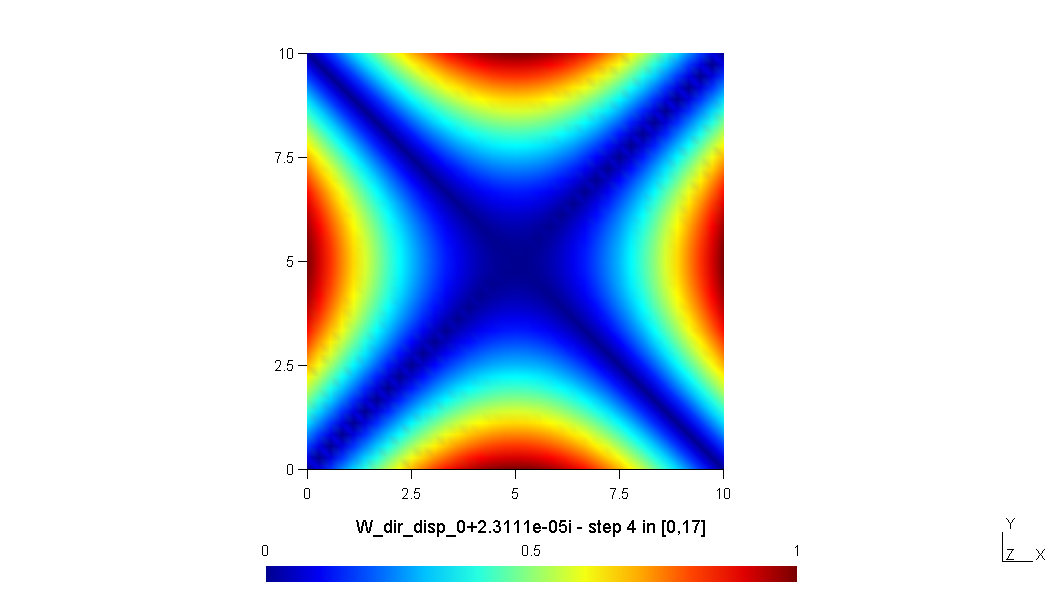
\includegraphics[width=\linewidth,trim={8cm 4cm 8cm 2cm},clip]{VMP09_T12_pos_F5.png}
%\caption{Mode Shape 5}
\end{subfigure}\hfill
\begin{subfigure}{.3\textwidth}
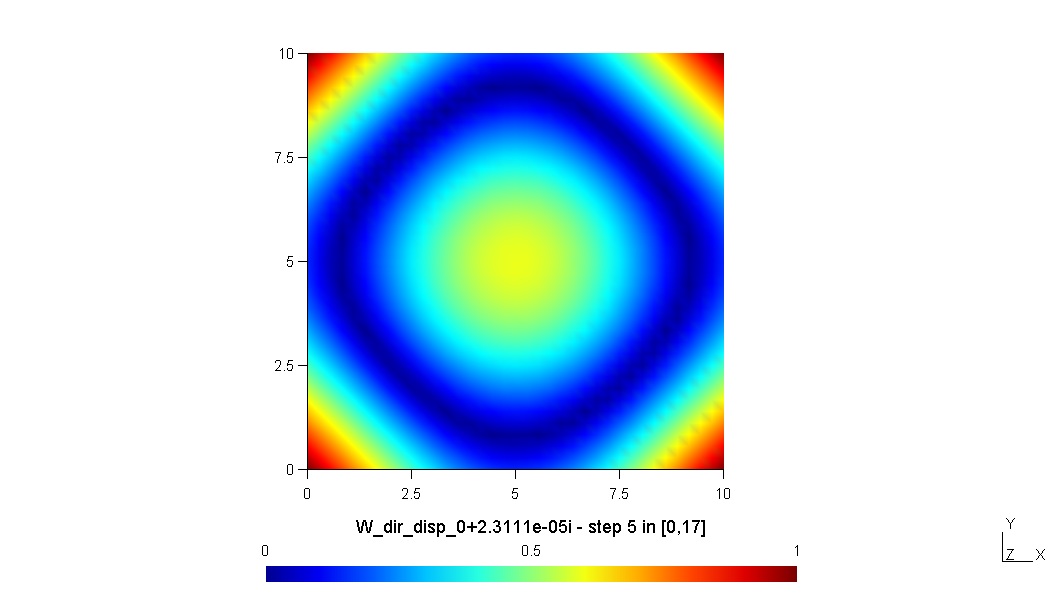
\includegraphics[width=\linewidth,trim={8cm 4cm 8cm 2cm},clip]{VMP09_T12_pos_F6.png}
%\caption{Mode Shape 6}
\end{subfigure}\vfill
\begin{subfigure}{.3\textwidth}
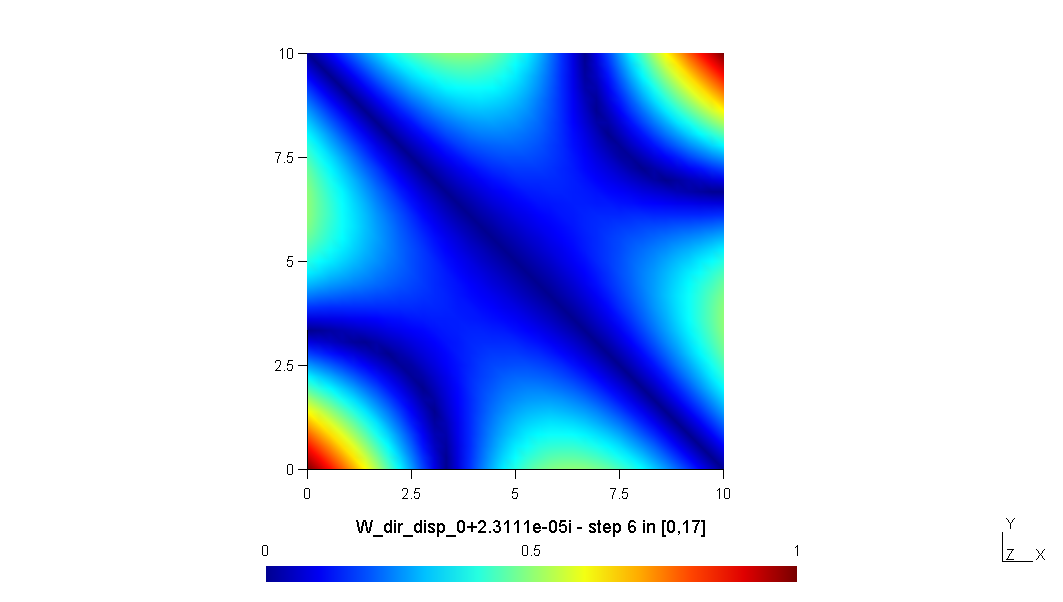
\includegraphics[width=\linewidth,trim={8cm 4cm 8cm 2cm},clip]{VMP09_T12_pos_F7.png}
%\caption{Mode Shape 7}
\end{subfigure} \hfill
\begin{subfigure}{.3\textwidth}
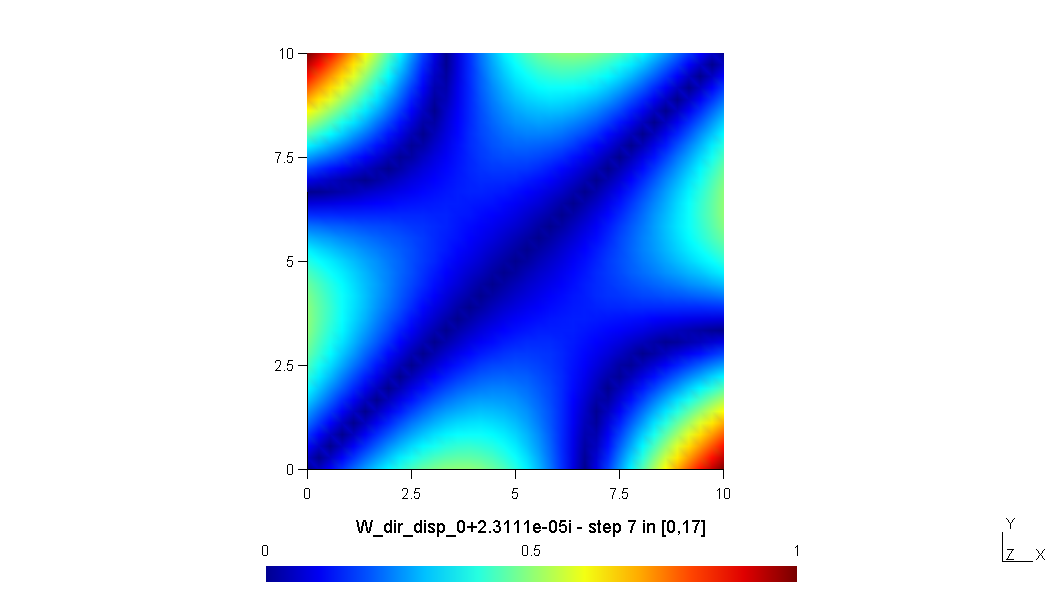
\includegraphics[width=\linewidth,trim={8cm 4cm 8cm 2cm},clip]{VMP09_T12_pos_F8.png}
%\caption{Mode Shape 8}
\end{subfigure}\hfill
\begin{subfigure}{.3\textwidth}
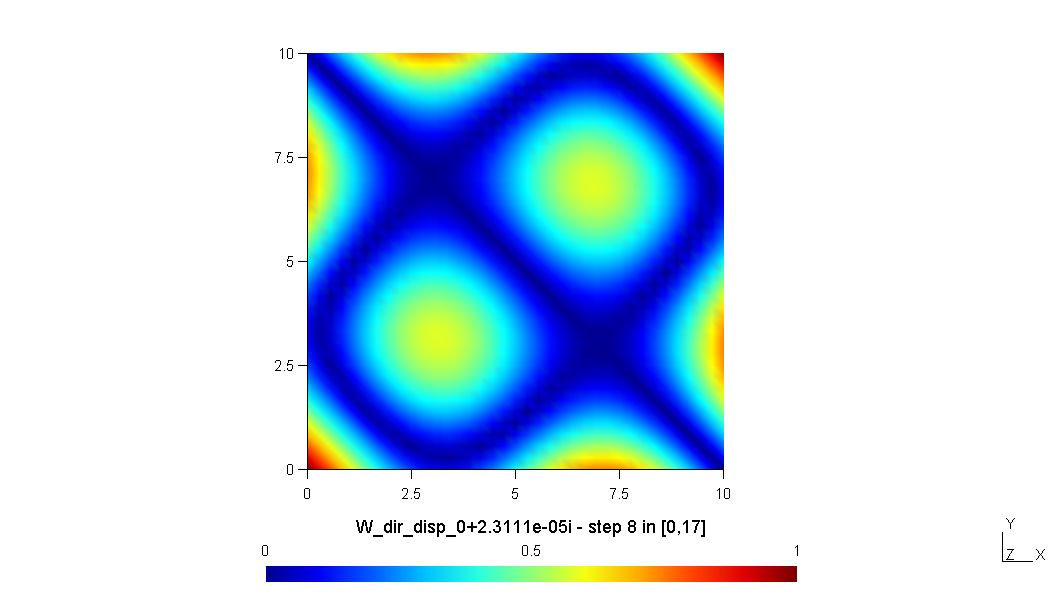
\includegraphics[width=\linewidth,trim={8cm 4cm 8cm 2cm},clip]{VMP09_T12_pos_F9.png}
%\caption{Mode Shape 9}
\end{subfigure}
%\caption{Natural Modes of a Square Plate}
\end{figure}

\begin{block}{Reference}
NAFEMS Manual. Solution Retrieved from Ansys verification problem (VMP09-T12).
\end{block}
Error $\%$ = 0.32 $\%$.



\end{frame}
\end{comment}


\begin{frame}
\frametitle{NAS227 Modal analysis of thin plate with axial load}

\begin{columns}
\column{0.5\textwidth}

\begin{figure}[h!]
\centering
\begin{subfigure}{1\textwidth}
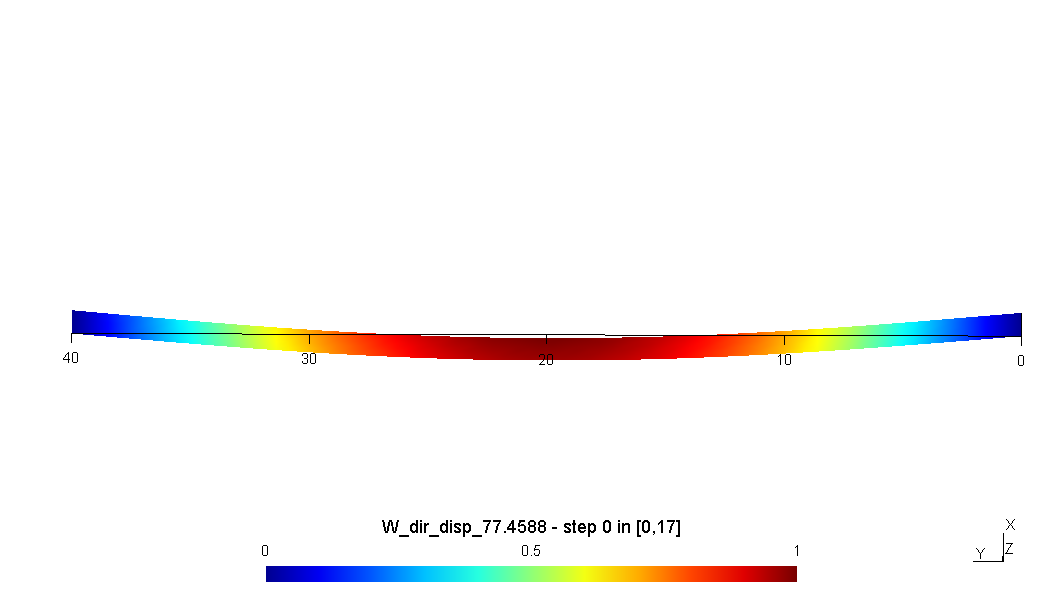
\includegraphics[width=\linewidth,trim={0 8cm 0 8cm},clip]{NAS277_pos_1.png}
%\caption{Mode Shape 1}
\end{subfigure} \vfill
\begin{subfigure}{1\textwidth}
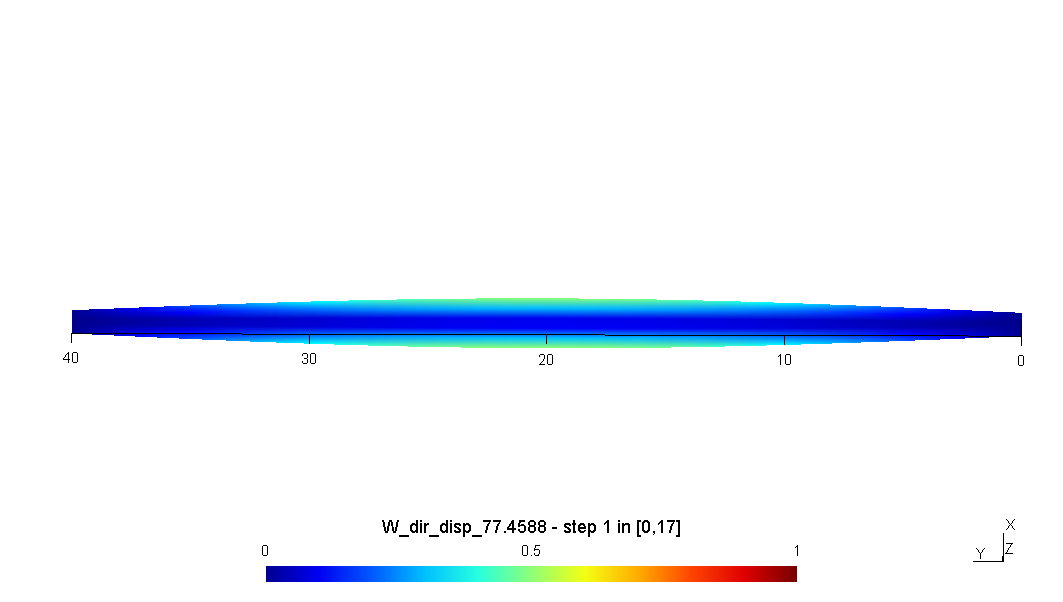
\includegraphics[width=\linewidth,trim={0 8cm 0 8cm},clip]{NAS277_pos_2.png}
%\caption{Mode Shape 2}
\end{subfigure}\vfill
\begin{subfigure}{1\textwidth}
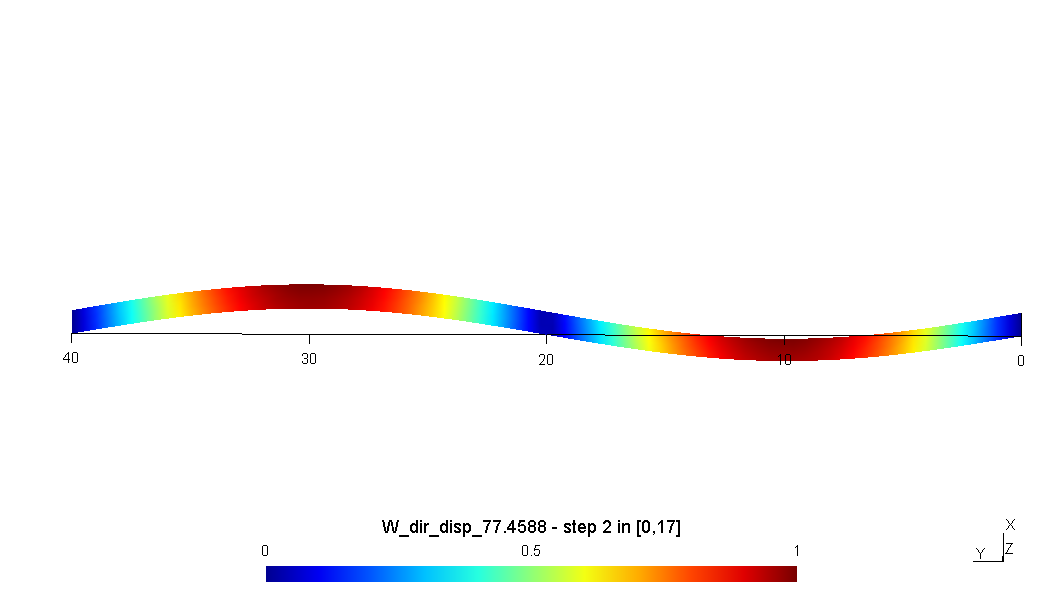
\includegraphics[width=\linewidth,trim={0 8cm 0 8cm},clip]{NAS277_pos_3.png}
%\caption{Mode Shape 3}
\end{subfigure}

%\caption{Natural Modes of a rectangular strip}
\end{figure}

Analytical Solution = 77.47 Hz \\
Numerical Solution =  77.45 Hz \\
Error $\%$ = 0.01 $\%$.


\begin{equation*}
\begin{split}
\rho^2 \omega_{mn}^2=   D  \left[ \left( \frac{m\pi}{a} \right)^2 + \left( \frac{n\pi}{b} \right)^2 \right]\\ + N_1 \left( \frac{m\pi}{a} \right)^2 +N_2 \left( \frac{n\pi}{b} \right)^2 
\end{split}
\end{equation*}



\column{0.5\textwidth}


\begin{table}[ht]
\renewcommand{\arraystretch}{1.5}
\centering
\begin{tabular}{ll}
\hline
\multicolumn{2}{l}{Material Property} \\ \hline  \hline
Young's Modulus ($E$)          &1E11 $Pa$        \\
Poission's Ratio ($\nu$)       & 0.3            \\ 
Density($\rho$)       &     7810         \\ 
    \hline
    \multicolumn{2}{l}{Geometric Data} \\ \hline  \hline
            length ($l$)        & 1 $m$   \\
            breath ($b$)        & 40 $m$   \\
            Thickness($t$)     &         0.5 $mm$  \\
             \hline
                \multicolumn{2}{l}{Loading Data} \\ \hline  \hline
            Axial load ($N_x$)        & 6E7 $N/m^2$   \\
             \hline
\end{tabular}
\end{table}






\end{columns}
\begin{block}{Reference}
Arthur W.Leissa ,Vibration of Plates,NASA SP-160, pg:277, Ch:10.2. \\
\end{block}
\end{frame}



\begin{comment}
\begin{frame}
\frametitle{Wave Speed in the moving metal strip}
The same model used in the previous problem is also used here with additional line speed to simulate moving material.

\begin{figure}[h!]
\centering
\begin{subfigure}{1\textwidth}
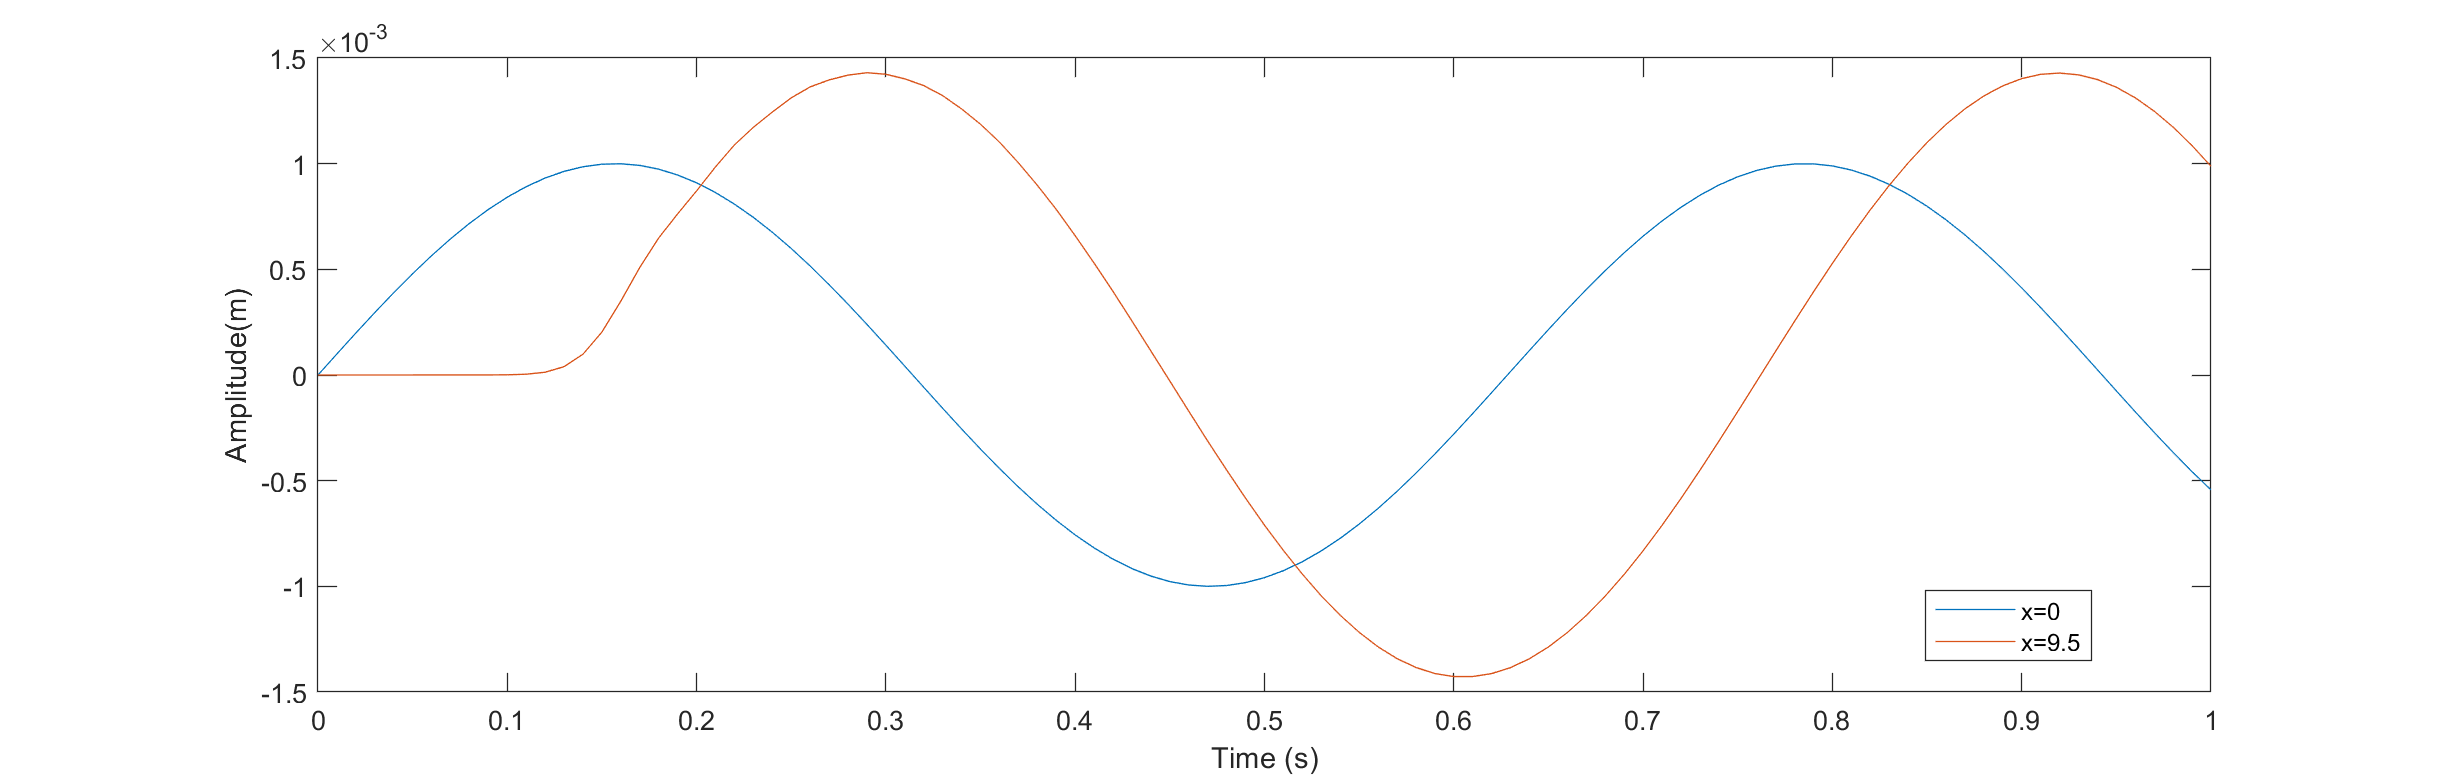
\includegraphics[width=\linewidth,trim={0 0 0 0},clip]{wavespeed.png}
%\caption{Mode Shape 1}
\end{subfigure} 

%\caption{Natural Modes of a rectangular strip}
\end{figure}
\begin{columns}

\column{0.5\textwidth}
\begin{equation*}
c=v+\sqrt{\frac{T}{m}}
\end{equation*}
 
 $T$ = Tension , $m$ = Mass per unit length, $v$ = line speed and $c$ = wave speed. 



\column{0.5\textwidth}

\begin{table}[ht]
\renewcommand{\arraystretch}{1.5}
\centering
\begin{tabular}{ll}
\hline
                \multicolumn{2}{l}{Loading Data} \\ \hline  \hline
            Line Speed ($V_1$)        &10 $m/s$   \\
             \hline
\end{tabular}
\end{table}
\end{columns}
Analytically Solution = 71.977 $ms^{-1}$, Numerical solution = 71.42 $ms^{-1}$ and The 
Error $\%$ = 0.89 $\%$.
\end{frame}

\begin{frame}
\frametitle{comparison with 1D FD model}
The same model is again employed to compare it with the existing one dimensional finite difference model.
\begin{figure}[h!]
\centering
\minipage{1\textwidth}%
  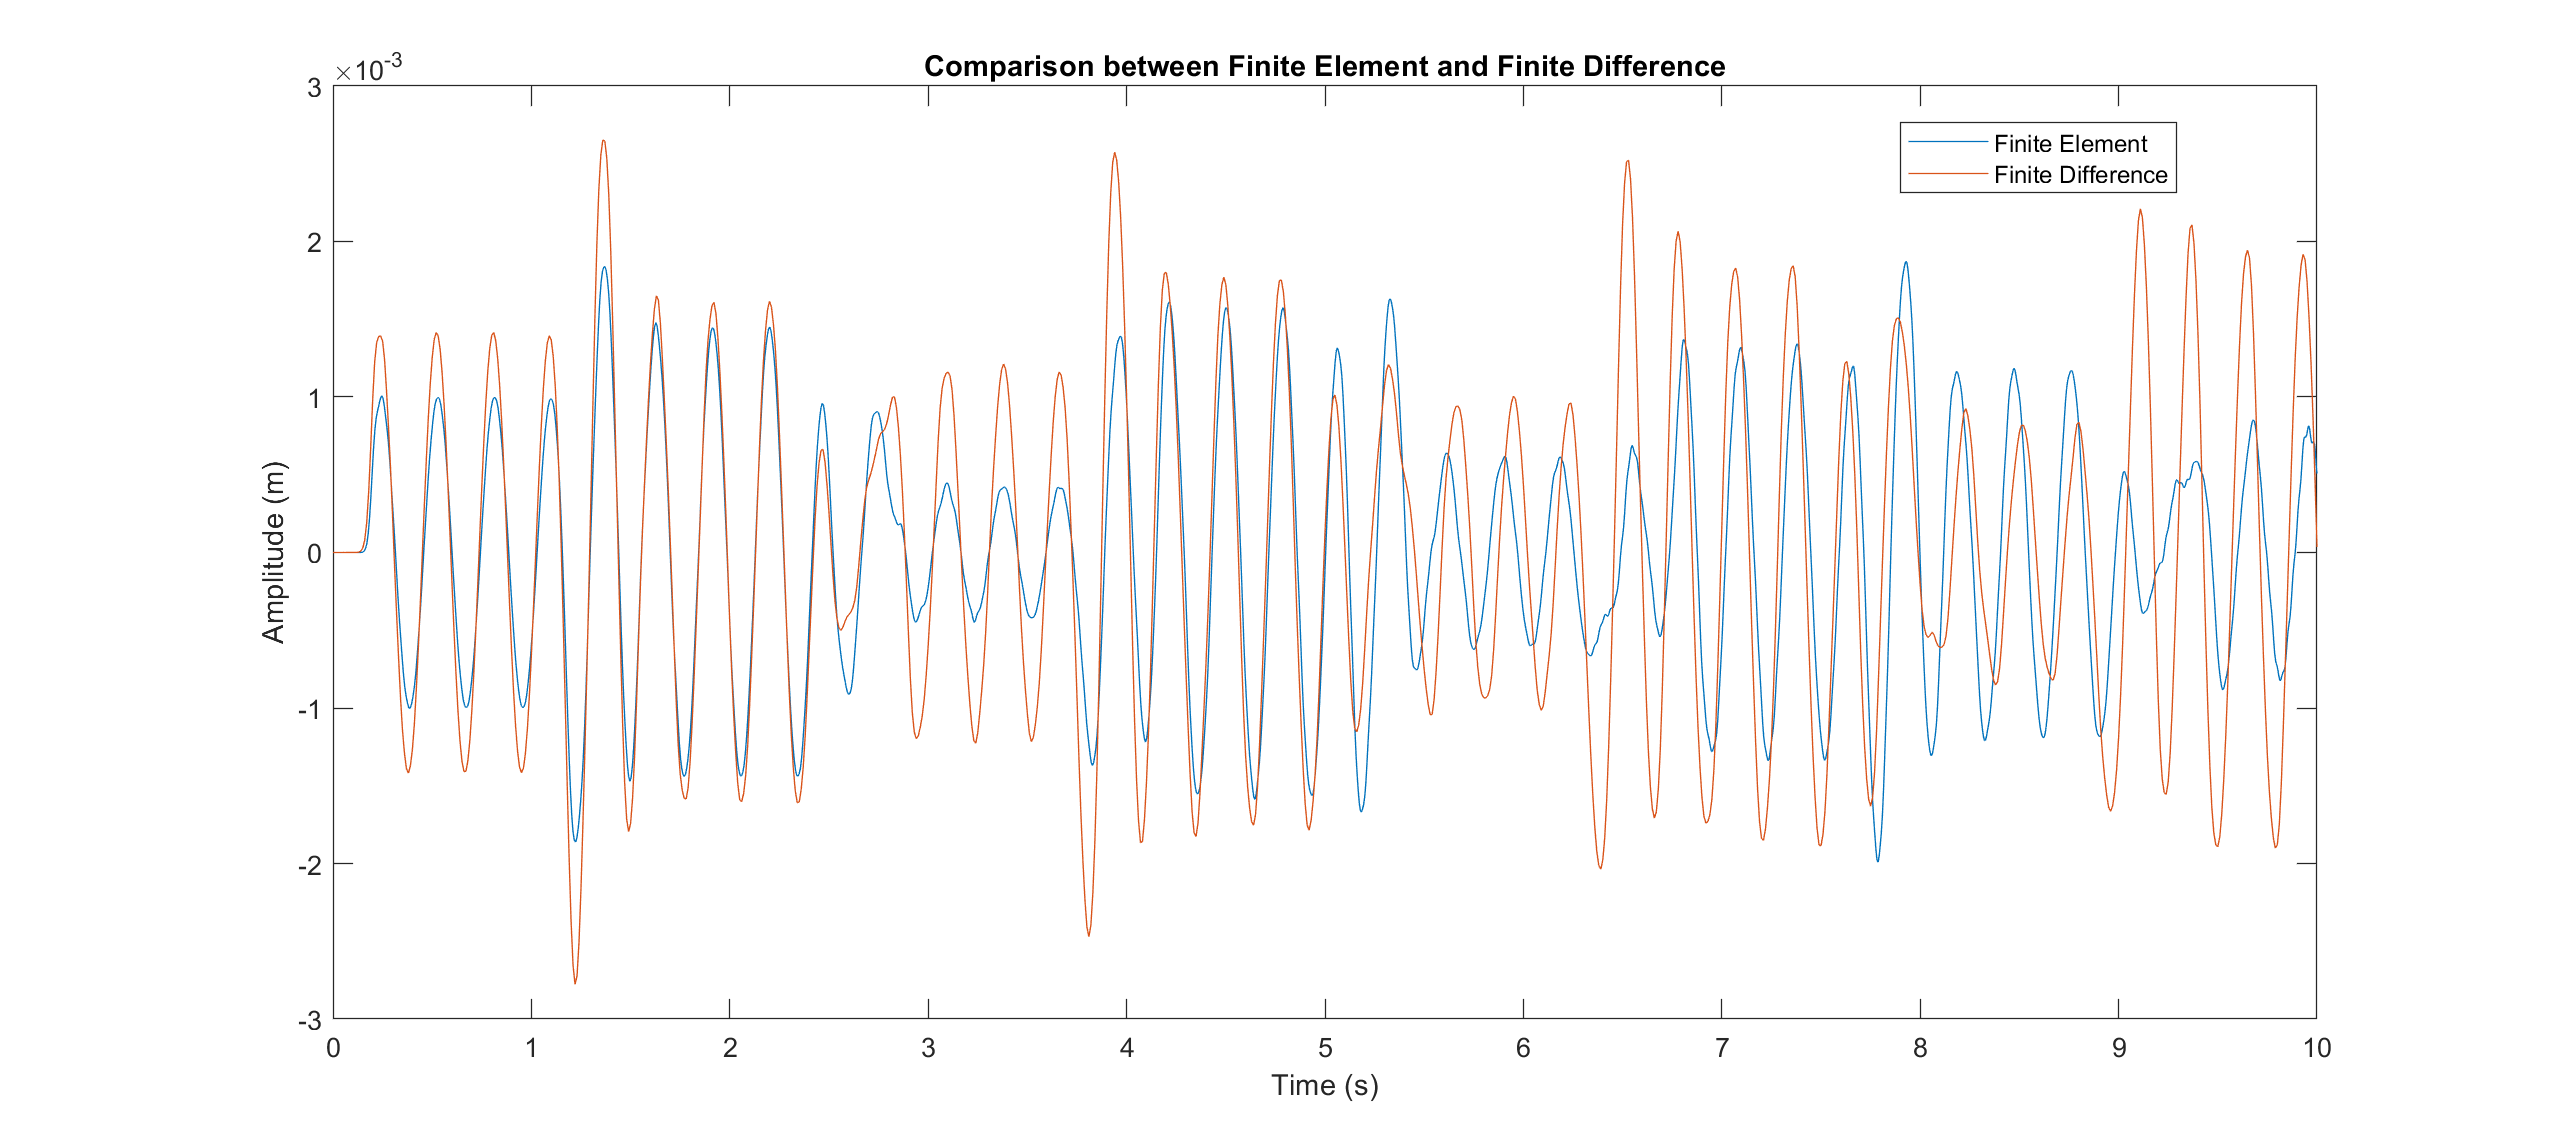
\includegraphics[width=\linewidth,trim={2cm 0 2cm 0},clip]{FdvsFe1.png}
  %\caption{FEM solution plot}\label{fig:awesome_image3}
\endminipage
\end{figure}
The displacement of the plate at the distance of 10 m from origin is plotted against time.
\end{frame}

\end{comment}

%\begin{frame}
%\frametitle{Mesh Dependency test 2}
%\begin{figure}[h!]
%\centering
%\subfile{galerkin.tex}
%\caption{NAS277} \label{NAS277sch}
%\end{figure}
%\end{frame}
%\section{Dynamic Simulation}

\begin{frame}
\frametitle{Comparison of FEM solution with Galerkin method }

\begin{figure}[h!]
\centering
\subfile{galcomp.tex}
%\caption{NAS277} \label{NAS277sch}
\end{figure}
\href{run:galcomp.mpg}{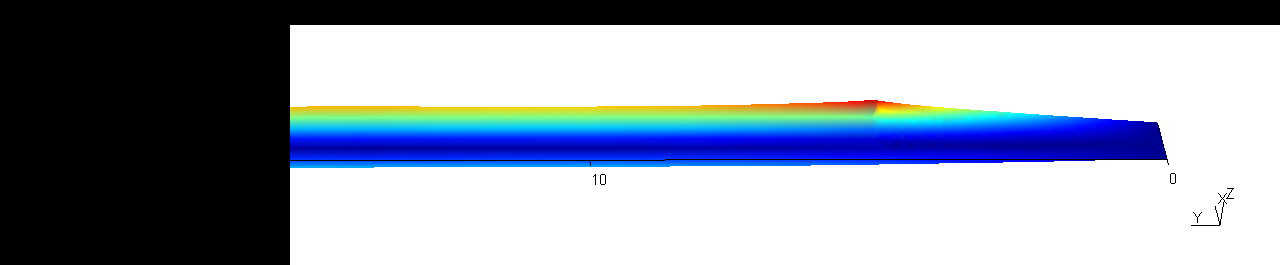
\includegraphics[width=1.0\textwidth,trim={10.5cm 0cm 0cm 2cm},clip]{galcomp.png}}



%\begin{block}{Analysis Statistics}
%nT=250 , nN = 1886 , nE = 1836, nDOF = 5640, Solution Time = s
%\end{block}

\end{frame}




\begin{frame}
\frametitle{Comparison of FEM solution with Galerkin method }
\begin{figure}[h!]
\centering
\subfile{FEMvsFDM.tex}
%\caption{NAS277} \label{NAS277sch}
\end{figure}

\end{frame}





\section{Dynamic Simulation}



\begin{frame}
%\frametitle{Some Dynamic analysis}
Same Geometry from previous problem with harmonic load at one end

\begin{figure}[h!]
\centering
\subfile{some_dyna_1.tex}
%\caption{NAS277} \label{NAS277sch}
\end{figure}
\href{run:movie1.mpg}{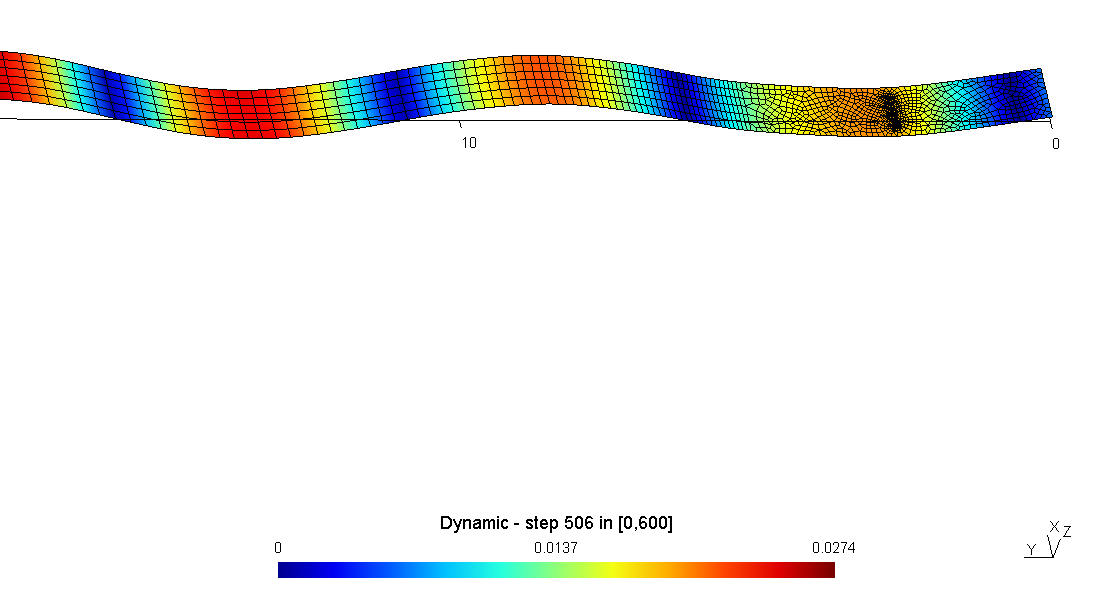
\includegraphics[width=1.0\textwidth,trim={0cm 15cm 0cm 1cm},clip]{ParaStudy_onlydata/dir.png}}



\begin{block}{Analysis Statistics}
nT=1000 , nN = 1886 , nE = 1836, nDOF = 5640, Solution Time = 145 s

\end{block}

\end{frame}


\begin{frame}
%\frametitle{Some Dynamic analysis}
Along with previous loading, forces are applied at designated spots.

\begin{figure}[h!]
\centering
\subfile{some_dyna_2.tex}
%\caption{NAS277} \label{NAS277sch}
\end{figure}
\href{run:movie2.mpg}{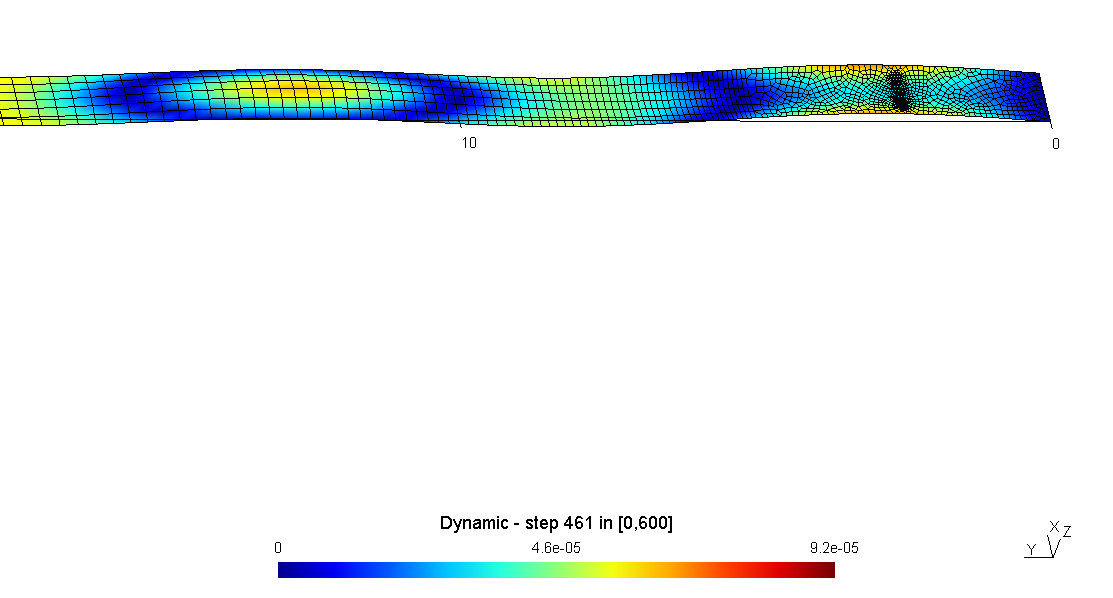
\includegraphics[width=1.0\textwidth,trim={0cm 15cm 0cm 1cm},clip]{ParaStudy_onlydata/for.png}}



\begin{block}{Analysis Statistics}
nT=1000 , nN = 1886 , nE = 1836, nDOF = 5640, Solution Time =182 s

\end{block}


\end{frame}





\begin{frame}
%\frametitle{Some Dynamic analysis}

Twisting deformation is applied at one end.

\begin{figure}[h!]
\centering
\subfile{some_dyna_3.tex}
%\caption{NAS277} \label{NAS277sch}
\end{figure}

\href{run:ParaStudy_onlydata/N2/3E7/Dynamic.mpg}{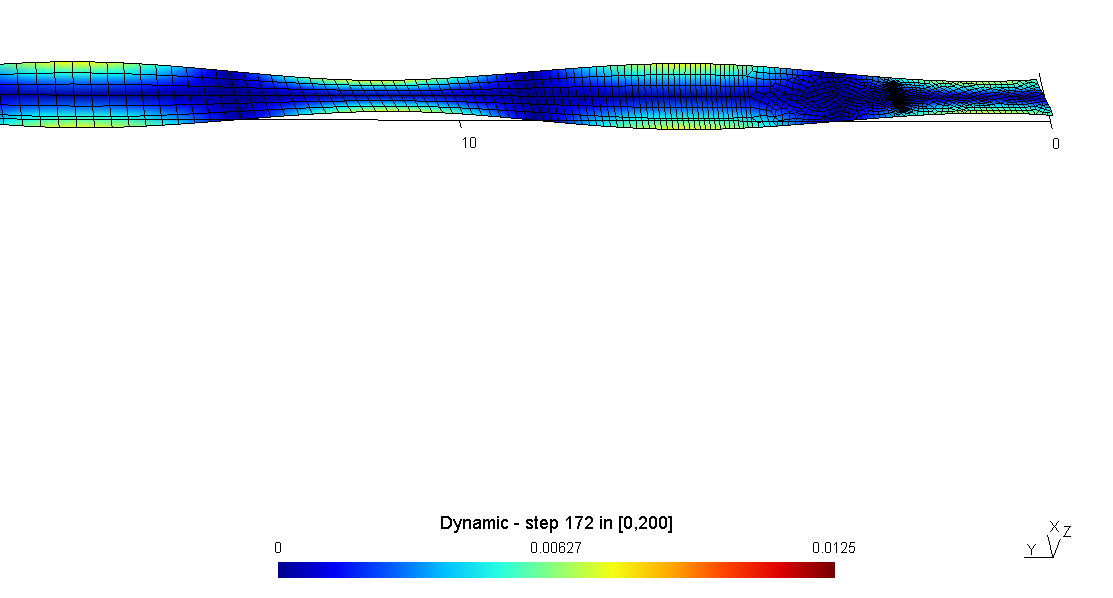
\includegraphics[width=1.0\textwidth,trim={0cm 15cm 0cm 1cm},clip]{ParaStudy_onlydata/twist.png}}


\begin{block}{Analysis Statistics}
nT=200 , nN = 1886 , nE = 1836, nDOF = 5640, Solution Time = 39s

\end{block}


\end{frame}







\begin{frame}
\frametitle{Response of the plate for different Axial velocities(V) $m/s $}
\begin{figure}[h!]
\centering
\subfile{Mesh_Para_study.tex}
%\caption{NAS277} \label{NAS277sch}
\end{figure}


\href{run:Young/1E11/Dynamic.mpg}{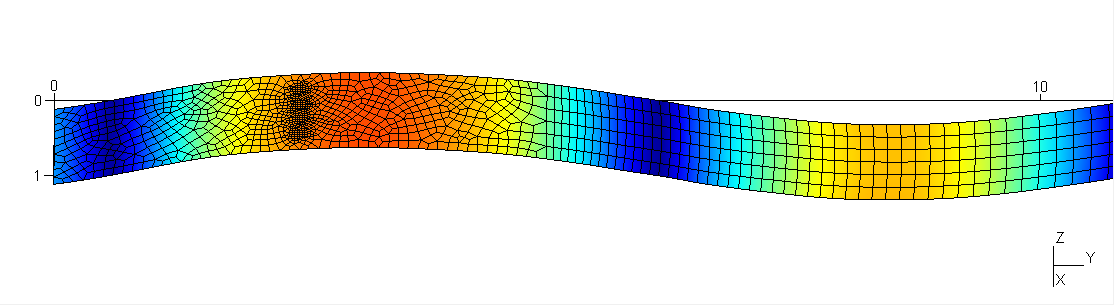
\includegraphics[width=1.0\textwidth,trim={0cm 0cm 0cm 0cm},clip]{ParaStudy_onlydata/Young/1E11/Dynamic.png}}



\end{frame}






\begin{frame}
\frametitle{Response of the plate for different Axial velocities(V) $m/s $}
\begin{figure}[h!]
\centering
%\subfile{ParaStudy_onlydata/V_Pn2.tex}
%\caption{NAS277} \label{NAS277sch}
\end{figure}
\end{frame}



\begin{frame}
\frametitle{Strip with displacement from real world data }
\begin{columns}

\column{0.8\textwidth}

\pgfplotsset{width=9cm,height=3cm,compat=1.16}
\begin{tikzpicture}
\begin{axis}[
%title= Plot of W displacement VS Time,
axis x line = bottom,
axis y line = left,
xlabel={$Time (s)$},
ylabel={w at y=0},
xmin=0, xmax=5,
%minor y tick num=1,
%legend pos=outer north east,
%cycle list name = color list,
%transpose legend,
%legend columns=3,
%legend style={at={(0.5,-0.1)},anchor=north},
]

%\addplot table{PN2.txt};
%\addplot [blue] table{1E11/Dynamic_Rad_Pn2.txt};
\addplot [blue] table{ParaStudy_onlydata/RandomLoad/Load2.txt};
%\addlegendentry{$SR$ = 1, ST = 2s}


\end{axis}
\end{tikzpicture}



\pgfplotsset{width=9cm,height=3cm,compat=1.16}
\begin{tikzpicture}
\begin{axis}[
%title= Plot of W displacement VS Time,
axis x line = bottom,
axis y line = left,
xlabel={$Time (s)$},
ylabel={w at y=0.5},
xmin=0, xmax=5,
%minor y tick num=1,
%legend pos=outer north east,
%cycle list name = color list,
%transpose legend,
%legend columns=3,
%legend style={at={(0.5,-0.1)},anchor=north},
]

%\addplot table{PN2.txt};
%\addplot [blue] table{1E11/Dynamic_Rad_Pn2.txt};
\addplot [blue] table{ParaStudy_onlydata/RandomLoad/Load1.txt};
%\addlegendentry{$SR$ = 1, ST = 2s}


\end{axis}
\end{tikzpicture}



\pgfplotsset{width=9cm,height=3cm,compat=1.16}
\begin{tikzpicture}
\begin{axis}[
%title= Plot of W displacement VS Time,
axis x line = bottom,
axis y line = left,
xlabel={$Time (s)$},
ylabel={w at y=1},
xmin=0, xmax=5,
%minor y tick num=1,
%legend pos=outer north east,
%cycle list name = color list,
%transpose legend,
%legend columns=3,
%legend style={at={(0.5,-0.1)},anchor=north},
]

%\addplot table{PN2.txt};
%\addplot [blue] table{1E11/Dynamic_Rad_Pn2.txt};
\addplot [blue] table{ParaStudy_onlydata/RandomLoad/Load3.txt};
%\addlegendentry{$SR$ = 1, ST = 2s}


\end{axis}
\end{tikzpicture}

\column{0.2\textwidth}
\href{run:ParaStudy_onlydata/RandomLoad/Dynamic_Rad1.mpg}{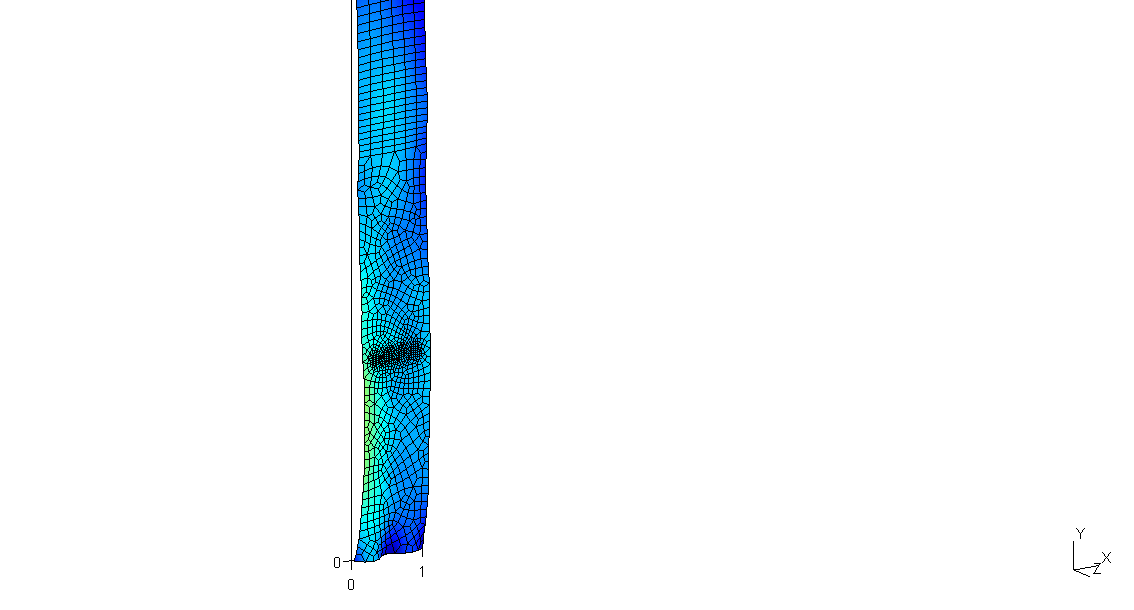
\includegraphics[width=1.0\textwidth,trim={11cm 0cm 22cm 0cm},clip]{ParaStudy_onlydata/RandomLoad/Dynamic_Rad1.png}}
\end{columns}
\end{frame}


\begin{frame}
\frametitle{Basic Control Demonstration}
\href{run:control_demo.mpg}{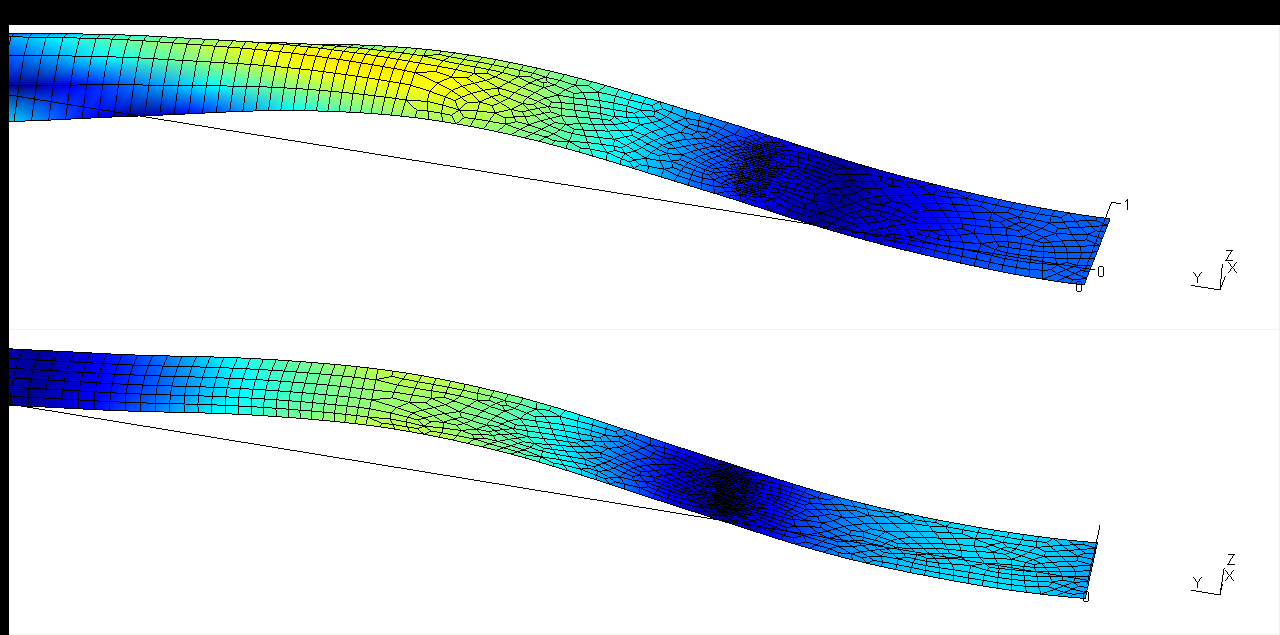
\includegraphics[width=1.0\textwidth,trim={0.5cm 11cm 0.1cm 1cm},clip]{control_demo.png}}

\begin{figure}[h!]
\centering
\subfile{control_demo.tex}
%\caption{NAS277} \label{NAS277sch}
\end{figure}

\end{frame}

\section{Conclusion}



\begin{frame}
\begin{block}{Work to be Done}
\begin{itemize}
\item Interfacing with control law
\item Optimizing the code to increase efficiency
\item To clear bugs and bottle necks
\item Creating well documentation for the FEM program.
\end{itemize}
\end{block}


%\begin{comment}
%\begin{block}{Possible Future work  To increase accuracy}
%\begin{itemize}
%\item Including some or all non-linearity
%\item Trying better shape functions
%\item Multi physics thermal, fluid ...
%\end{itemize}
%\end{block}
%\begin{block}{Possible Future work  To increase efficiency}
%\begin{itemize}
%\item Better LAPLACK packages
%\item graphics acceleration using CULAB package
%\item Modal order reduction techniques
%\item Modal superposition technique
%\end{itemize}
%\end{block}
%\end{comment}


\begin{block}{Suggested Future Work}
\begin{itemize}
\item Better Shape function
\item Including non-linearity and Multi physics
\item Including Contact between plate and rollers
\item Better Linear algebra solver packages (LAPACK, cuBLAS ..)
\item Modal superposition and Modal order reduction  techniques
\item Creating a user friendly GUI
\end{itemize}
\end{block}

\end{frame}



\begin{frame}
\frametitle{Conclusion}
\begin{block}{Advantages of FEM}
\begin{itemize}
\item Better control over accuracy.
\item Once coded successfully, It is very easy to implement even for complex geometry and mesh.
\item Higher dimensions can be easily modelled.
\end{itemize}

\end{block}

\begin{block}{Disadvantages of FEM}
\begin{itemize}
\item Computationally expensive.
\item Complexity in coding may be overwhelming .
\item Suffers from "The curse of dimensionality!".

\end{itemize}

\end{block}
\end{frame}

\begin{frame}
\begin{center}
\begin{LARGE}
\textbf{Thank you for your attention!!!}
\end{LARGE}
\end{center}


\end{frame}

\end{document}
